%% Manuscript for Mechanical Systems and Signal Processing (Elsevier).
%% Build: latexmk -pdf main.tex
\documentclass[preprint,12pt]{elsarticle}

\usepackage[T1]{fontenc}
\usepackage{lmodern}
\usepackage{amsmath,amssymb,amsthm}
\usepackage{bm}
\usepackage{graphicx}
\usepackage{booktabs}
\usepackage{array}
\usepackage{multirow}
\usepackage{siunitx}
\sisetup{detect-all, range-phrase={--}, range-units=single, per-mode=symbol, group-minimum-digits=5}
\DeclareSIUnit\rpm{rpm}
\usepackage{tikz}
\usetikzlibrary{arrows.meta,positioning,calc}
\usepackage{xcolor}
\usepackage[hidelinks]{hyperref}
\pdfstringdefDisableCommands{\def\corref#1{}}
\usepackage{lineno}
\usepackage{flafter}
\renewcommand{\topfraction}{0.85}
\renewcommand{\bottomfraction}{0.6}
\renewcommand{\textfraction}{0.12}
\renewcommand{\floatpagefraction}{0.75}
\setcounter{topnumber}{3}
\setcounter{totalnumber}{4}

\biboptions{numbers,sort&compress}
\journal{Mechanical Systems and Signal Processing}

\newtheorem{lemma}{Lemma}
\newtheorem{proposition}{Proposition}
\newtheorem{remark}{Remark}
\hyphenation{bi-stable bi-stab-il-ity}
\newcommand{\sat}{\operatorname{sat}}
\newcommand{\alim}{a_{\lim}}
\newcommand{\achk}{a_{\mathrm{chk}}}
\newcommand{\Vmax}{V_{\max}}
\newcommand{\bmax}{b_{\max}}
%% DRAFT-PLACEHOLDERS-BEGIN
\newcommand{\PEND}[1]{\textbf{[#1]}}
%% DRAFT-PLACEHOLDERS-END

\begin{document}

\begin{frontmatter}

\title{Beyond linear stability lobes: saturation-induced finite-amplitude instability and basin-aware gain scheduling in actively damped milling}

%% Authors and affiliations: to be completed by the authors.
\author[a]{[Author name]\corref{cor1}}
\ead{[corresponding e-mail]}
\cortext[cor1]{Corresponding author.}
\affiliation[a]{organization={[Department, Institution]},
            city={[City]},
            country={[Country]}}

\begin{abstract}
Linear stability lobes can overestimate the usable depth of cut when an active damping actuator saturates. This computational study asks how much disturbance a linearly stable milling cut with voltage-limited velocity feedback tolerates before saturation triggers chatter. In a single-mode model of a published case study (17 of 19 tests classified as measured), the command splits into a forced part and the residual authority left for disturbances, which governs the basin near the limit. An abrupt entry chatters below 97\,\% of the linear limit at 157 of 251 speeds; near the limit, kicks of 2.4--10.8\,\% of one tooth's cutting impulse end in bounded clipped chatter coexisting with the stable cut. A circle criterion, its frequency condition proved by interval arithmetic, shows the forced orbit of the averaged delay model to attract every solution below a depth whose median is 0.97 of the uncontrolled limit; above it, linear matrix inequalities give inner estimates of the basin, numerically verified for collocation models and never violated in simulation. A basin-aware gain schedule, searched on grids at 21 speeds, gives the largest depth that is linearly stable, keeps a voltage margin and is certified against a required disturbance. With equal gain range and margins its gains certify 6\,mm more depth than authority-based ones for 5\,mm/s, hardly more for 1\,mm/s; with abrupt entry or a 16\,mm cap it cuts no deeper. Under sampled model errors its points, nearer their linear limit, fail more often (10--17\,\% against 7\,\%).

\end{abstract}

\begin{highlights}
\item Actuator saturation makes linearly stable milling cuts bistable with clipped chatter
\item Step entries from rest chatter below 0.97 of the linear limit at 157 of 251 speeds
\item Residual actuator authority sets the basin of the forced orbit near the limit
\item Circle criterion and LMIs bound the basin of the averaged and collocation models
\item A basin-aware gain schedule certifies model depths against a required disturbance
\end{highlights}

\begin{keyword}
Milling chatter \sep Active damping \sep Actuator saturation \sep Finite-amplitude instability \sep Basin of attraction \sep Linear matrix inequalities \sep Gain scheduling
\end{keyword}

\end{frontmatter}

\linenumbers

\section{Introduction}\label{sec:intro}

Regenerative chatter limits the material removal rate of most milling operations. Its linear mechanism, the delayed feedback of the surface left by the previous tooth, is captured by stability lobe diagrams computed in the frequency domain with the zero-order approximation \citep{altintas1995analytical} or in the time domain with semi-discretisation and related methods \citep{insperger2002semi,insperger2004updated,insperger2011book}; see the reviews of \citet{quintana2011chatter}, \citet{munoa2016chatter} and \citet{altintas2020chatter}. Among the suppression techniques, active damping adds a controlled force to the machine or the workpiece. Proof-mass (inertial) actuators driven by direct velocity feedback (DVF) are attractive because the loop is simple and collocated: with an ideal force actuator it is unconditionally stable, and with an inertial actuator it is stable up to a gain set by the actuator's own resonance \citep{elliott2001feedback}; active damping of milling chatter with such actuators and with related structural actuators has been demonstrated on laboratory set-ups and machine tools \citep{dohner2004mitigation,munoa2013chatter,vandijk2012robust,monnin2014optimal}.

The weak point of an inertial actuator is the force it can deliver. A stroke-limited inertial actuator in a velocity feedback loop damps small vibrations and can lose stability at large ones, which gives rise to limit cycles \citep{baumann2007destabilization}. In milling the actuator has to provide two forces at once: the force that damps the chatter mode, and the force that the feedback reacts with against the forced, tooth-periodic vibration of a stable cut. \citet{ozsoy2025frequency} modelled actuator saturation in the frequency domain, and \citet{ozsoy2026robust} proposed a saturation-aware gain map: at each spindle speed, the DVF gain that maximises the linear stability limit subject to the peak force demand of a simulated cut staying within the actuator capacity. Their study is the starting point of the present one.

Saturation turns the controlled cut into a nonlinear system, and nonlinear chatter has a long history. Loss of contact between tool and workpiece bounds the chatter amplitude \citep{tlusty1981basic}, the Hopf bifurcation of the regenerative model is subcritical \citep{kalmarnagy2001subcritical,stepan2005nonlinear}, and linearly stable cuts coexist with chatter in bistable, or unsafe, zones below the linear limit \citep{dombovari2015bistable}. Bistability of turning under active velocity feedback damping has been analysed by \citet{sahu2021bistability}. For chatter controllers designed with input constraints, regional guarantees around the chatter-free motion have been given as ellipsoidal invariant sets of a predictive controller \citep{zhang2015ellipsoid} and as positively invariant sets of an adaptive controller with hard input clipping \citep{wu2016adaptive}. The tools for such guarantees come from the analysis of linear systems with saturating inputs: sector conditions that bound the dead-zone nonlinearity locally and give ellipsoidal estimates of the region of attraction through linear matrix inequalities (LMIs) \citep{hu2001book,gomesdasilva2005antiwindup,tarbouriech2011book}, extended to periodic systems with periodic or clock-dependent Lyapunov functions \citep{allerhand2011robust,briat2013clock,li2015periodic,zhou2011periodic,yang2015periodic}. Delay equations are commonly turned into ordinary differential equations of finite order by spectral collocation of the delayed history \citep{breda2005pseudospectral,breda2015book}, an approach also used for the periodic milling equation \citep{butcher2009chebyshev}.

A second line of work reduces the control effort itself. A delayed feedback of the form $\dot x(t)-\dot x(t-T)$ vanishes on every motion with period $T$ \citep{pyragas1992continuous}; in machining, controllers built on the difference between the present and the delayed motion have been used to shape the stability limit \citep{vandewouw2015ifac,vandijk2015ijrnc}, to counter the regenerative effect in turning \citep{mancisidor2019mechatronics}, and to obtain stability with less control effort \citep{li2022ijamt,du2024ijms}. Such a term would spend none of the actuator's authority on the forced vibration of a stable cut, which is exactly the share that a saturation-aware DVF design has to budget.

What remains open, for a fixed DVF law whose command is clipped at the actuator capacity in a regenerative milling model, is (i) how the authority condition of a saturation-aware gain map should be posed so that it is well defined, (ii) whether and by how much the clip makes the linearly stable cut bistable across the speed range, and how this depends on the way the tool enters the cut, (iii) how large a basin around the forced orbit can be guaranteed when part of the authority is spent on the forced vibration, and (iv) whether a delayed term that spends no authority on the forced orbit enlarges the basin, and at what cost in robustness. This paper addresses these four questions on the case study of \citet{ozsoy2026robust}. Its contributions are:
\begin{enumerate}
\item A well-posed authority condition (Section~\ref{sec:feasibility}). The published test takes the peak demand of a simulation that starts from rest, which is set by the entry transient and makes the feasible set of gains fragmented. The condition proposed here bounds the steady forced demand in closed form at every depth up to a margin below the limit and checks the result in the time domain with the clipped actuator.
\item A map of saturation-induced bistability for the clipped DVF loop over 251 spindle speeds (Section~\ref{sec:bistability}): the dependence of the attainable depth on the entry, the lower edge of the bistable band, and the size of the basin measured by velocity kicks, with and without the clip, in a simulator that remembers the full machined surface.
\item Certificates of the basin (Section~\ref{sec:certificates}): ellipsoidal sets around the forced orbit proved by sector-condition LMIs in which the dead zone moves with the forced command, so that the authority spent on the forced vibration enters the certificate, first on a collocation model of the averaged milling model and then on one of the time-periodic model, each solution checked independently of the solver and validated against the simulator.
\item An analysis of the authority-preserving delayed term under the same hard clip and the same authority rule as DVF (Section~\ref{sec:delayed}): linear limits, simulated entries, certified basins, and the robustness limits set by loop delay, unmodelled modes, delay mismatch and runout.
\end{enumerate}
The tools are not new: the bistable zone, sector conditions, collocation and the delayed difference law are all established. The contribution is their combination for this problem, the quantification over the speed range, and the cross-validation of the certificates against an independent simulator. The study is computational; Section~\ref{sec:discussion} discusses what an experimental validation would need. Section~\ref{sec:model} introduces the model and the case study, and Section~\ref{sec:conclusions} concludes.

\section{Model and case study}\label{sec:model}

The model is the actively damped milling system of \citet{ozsoy2026robust}, rebuilt from its published parameters; Fig.~\ref{fig:model} shows the loop. This section states the equations used in all later sections: the clipped feedback loop, the regenerative force of the helical cutter, the linear stability limit and the tooth-periodic forced orbit.

\begin{figure}[t]
\centering
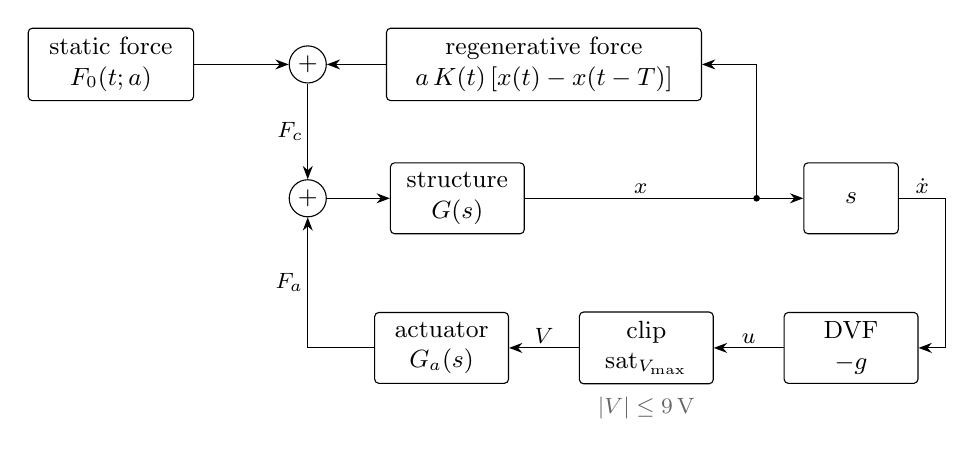
\begin{tikzpicture}[
  >=Stealth, font=\small,
  blk/.style={draw, rounded corners=1.5pt, minimum height=9mm, align=center, fill=white},
  sum/.style={draw, circle, inner sep=1.4pt, fill=white},
  lab/.style={font=\footnotesize, inner sep=1.5pt}]
  % junctions and blocks, placed explicitly so that no wire crosses a block
  \node[sum] (s1) at (0,0) {$+$};
  \node[sum] (s2) at (0,1.7) {$+$};
  \node[blk, minimum width=21mm] (F0) at (-2.5,1.7) {static force\\ $F_0(t;a)$};
  \node[blk, minimum width=40mm] (cut) at (3.0,1.7) {regenerative force\\ $a\,K(t)\,[x(t)-x(t-T)]$};
  \node[blk, minimum width=17mm] (G) at (1.9,0) {structure\\ $G(s)$};
  \node[coordinate] (xb) at (5.7,0) {};
  \node[blk, minimum width=12mm] (D) at (6.9,0) {$s$};
  \node[coordinate] (vb) at (8.1,0) {};
  \node[blk, minimum width=17mm] (K) at (6.9,-1.9) {DVF\\ $-g$};
  \node[blk, minimum width=17mm] (sat) at (4.3,-1.9) {clip\\ $\sat_{\Vmax}$};
  \node[blk, minimum width=17mm] (Ga) at (1.7,-1.9) {actuator\\ $G_a(s)$};
  % cutting forces
  \draw[->] (F0.east) -- (s2.west);
  \draw[->] (cut.west) -- (s2.east);
  \draw[->] (s2.south) -- node[lab, left] {$F_c$} (s1.north);
  % structure and velocity
  \draw[->] (s1.east) -- (G.west);
  \draw (G.east) -- node[lab, above, pos=0.5] {$x$} (xb);
  \fill (xb) circle (1.2pt);
  \draw[->] (xb) -- (D.west);
  \draw[->] (xb) |- (cut.east);
  \draw (D.east) -- node[lab, above] {$\dot x$} (vb);
  % feedback loop
  \draw[->] (vb) |- (K.east);
  \draw[->] (K.west) -- node[lab, above] {$u$} (sat.east);
  \draw[->] (sat.west) -- node[lab, above] {$V$} (Ga.east);
  \draw[->] (Ga.west) -| node[lab, left, pos=0.75] {$F_a$} (s1.south);
  \node[lab, below=1mm of sat, text=black!60] {$|V|\le\SI{9}{\volt}$};
\end{tikzpicture}
\caption{The controlled cut. The workpiece mode $G(s)$ is driven by the cutting force $F_c$, made of a static, tooth-periodic part and a regenerative part proportional to $x(t)-x(t-T)$, and by the force $F_a$ of the proof-mass actuator. The direct velocity feedback command $u=-g\dot x$ is clipped at $\Vmax=F_{\max}/K_a=\SI{9}{\volt}$. In Section~\ref{sec:delayed} the DVF block is replaced by the delayed difference law of Eq.~\eqref{eq:comb-law}.}
\label{fig:model}
\end{figure}


\subsection{Structure, actuator and clipped velocity feedback}\label{sec:model-loop}

The workpiece is flexible in one direction, normal to the feed, and is represented by its dominant mode. With $x(t)$ the displacement at the cutting point and $q(t)$ the internal coordinate of the proof-mass actuator,
\begin{equation}\label{eq:eom}
  m\ddot x+c\dot x+kx=f_c(t)+f_a(t),\qquad
  \ddot q+2\zeta_a\omega_a\dot q+\omega_a^2q=V(t),\qquad
  f_a=K_a\ddot q ,
\end{equation}
where $f_c$ is the cutting force on the workpiece and $f_a$ the actuator force. The structure and the actuator thus have the transfer functions $G(s)=1/(ms^2+cs+k)$ and $G_a(s)=K_as^2/(s^2+2\zeta_a\omega_as+\omega_a^2)$, the latter in newtons per volt. The actuator mode lies at $\omega_a/2\pi=\SI{8.40}{\hertz}$ with $\zeta_a=0.150$; at \SI{129.3}{\hertz} the magnitude of $G_a$ is within \SI{0.4}{\percent} of $K_a$ and its phase is \SI{1.1}{\degree}. The controller is direct velocity feedback (DVF) through this inertial actuator \citep{elliott2001feedback}, $u(t)=-g\dot x(t)$, and the applied command is clipped:
\begin{equation}\label{eq:dvf}
  V(t)=\operatorname{sat}_{V_{\max}}\bigl(u(t)\bigr)=\max\bigl\{-V_{\max},\,\min\{V_{\max},u(t)\}\bigr\},
\end{equation}
with $V_{\max}=F_{\max}/K_a=\SI{9}{\volt}$. While the clip is inactive the loop is linear, with the closed-loop receptance
\begin{equation}\label{eq:Gcl}
  G_{\mathrm{cl}}(s)=\frac{G(s)}{1+g\,s\,G_a(s)\,G(s)} .
\end{equation}
At $g=\SI{1500}{\volt\second\per\metre}$ the structural pole of Eq.~\eqref{eq:Gcl} has \SI{15.1}{\percent} damping at \SI{128.97}{\hertz}, against \SI{1.34}{\percent} without control, and the actuator pole has \SI{14.1}{\percent}. The clip acts on the command, before the actuator dynamics, so the force produced can transiently exceed $F_{\max}$ (up to \SI{29.5}{\newton} in the step entries at $g=1500$). Clipping at \SI{8.1}{\volt} instead, which keeps the force below \SI{27}{\newton}, lowers the clipped step-entry limits at $g=1500$ from 13.01 to \SI{12.47}{\milli\metre} at \SI{2500}{\rpm} and from 12.79 to \SI{12.10}{\milli\metre} at \SI{3000}{\rpm}.
% src: src/params.py, src/structure.py; verification/zoa_sdm/actuator_mode.json (|Ga|/K_a = 1.004 and 1.12 deg at 129.3 Hz; poles at g = 1500: 128.97 Hz, 15.07 %, and 8.42 Hz, 14.14 %); README §4.6 (clip before the actuator); verification/paper/support_runs.json (clip: 13.01/12.47 mm at 2500 rpm, 12.79/12.10 mm at 3000 rpm for 9/8.1 V; peak actuator force 29.5/26.6 N)

\subsection{Regenerative force of the helical cutter}\label{sec:model-force}

The cutter has $N_t=4$ teeth, radius $R=D/2$ and helix angle $\eta$. The immersion angle of tooth $j$ at height $z\in[0,a]$ above the tool tip is
\begin{equation}\label{eq:phi}
  \phi_j(t,z)=\Omega t+2\pi j/N_t-z\tan\eta/R ,\qquad j=0,\dots,N_t-1,
\end{equation}
measured clockwise from the feed-normal direction; in half-immersion down milling a tooth cuts while $\phi_j\in[\phi_{\mathrm{st}},\phi_{\mathrm{ex}}]=[\pi/2,\pi]$ (modulo $2\pi$), which is indicated by $\gamma_j(t,z)=1$ ($\gamma_j=0$ otherwise). The chip thickness of the slice $\mathrm dz$ is
\begin{equation}\label{eq:chip}
  h_j(t,z)=f_z\sin\phi_j-\bigl[x(t)-x(t-T)\bigr]\cos\phi_j ,
\end{equation}
the surface having been left by the preceding tooth one tooth period $T$ earlier. \ref{app:simulator} replaces $x(t-T)$ by the deepest earlier pass, which matters once the tool leaves the cut. The force on the workpiece along $x$ is
\begin{equation}\label{eq:fcut}
  f_c(t)=-\sum_{j=0}^{N_t-1}\int_0^a\gamma_j\,\bigl(K_{tc}\sin\phi_j-K_{rc}\cos\phi_j\bigr)\max\{h_j,0\}\,\mathrm dz ,
\end{equation}
so the force vanishes where the tool loses contact. As long as every engaged chip is positive, $f_c$ splits into a static and a regenerative part,
\begin{align}
  f_c(t)&=f_s(t;a)+aH(t)\,\bigl[x(t)-x(t-T)\bigr],\label{eq:split}\\
  aH(t)&=\sum_{j=0}^{N_t-1}\int_0^a\gamma_j\,\bigl(K_{tc}\sin\phi_j\cos\phi_j-K_{rc}\cos^2\phi_j\bigr)\,\mathrm dz ,\label{eq:aHt}
\end{align}
where $f_s$ is Eq.~\eqref{eq:fcut} with $h_j=f_z\sin\phi_j$. Both $f_s$ and the coefficient $aH(t)$ are $T$-periodic. Over one tooth period every axial slice contributes the same mean, only shifted in time by the helix, so the mean coefficient is exactly linear in the depth \citep{altintas1995analytical}:
\begin{equation}\label{eq:aHmean}
  \begin{aligned}
    \overline{aH}&=\frac{N_tK_{tc}\,a}{4\pi}\,\alpha_{yy},\\
    \alpha_{yy}&=2\int_{\pi/2}^{\pi}\Bigl(\sin\phi\cos\phi-\frac{K_{rc}}{K_{tc}}\cos^2\phi\Bigr)\mathrm d\phi
    =-1-\frac{\pi}{2}\,\frac{K_{rc}}{K_{tc}}=-1.428 ,
  \end{aligned}
\end{equation}
with $\alpha_{yy}$ the directional factor of the feed-normal direction. The axial tooth pitch $p_a=2\pi R/(N_t\tan\eta)=\SI{12.57}{\milli\metre}$ is comparable with the depths of interest, so the helix cancels most of the variation of $aH(t)$: near the stability limit it stays within about $\pm\SI{12}{\percent}$ of its mean, more at shallow depths, and it is constant when $a$ is a multiple of $p_a$ \citep{zatarain2006helix,insperger2006helix}.
% src: src/zoa.py (alpha_matrix), src/tdsim.c (force), src/c3_periodic.py (aH); verification/zoa_sdm/README.md §1 (derivation, alpha_yy = -1.428399); README §12.2 (+-12 % near the limit), §14.4 (pitch)

\subsection{Linear stability limit}\label{sec:model-zoa}

Replacing $aH(t)$ by its mean, Eq.~\eqref{eq:aHmean}, which is the zero-order approximation (ZOA) of \citet{altintas1995analytical}, and linearising the deviation from the forced orbit of Section~\ref{sec:model-orbit} gives the characteristic equation
\begin{equation}\label{eq:char}
  1-\frac{N_tK_{tc}\,a}{4\pi}\,\alpha_{yy}\bigl(1-e^{-i\omega T}\bigr)\,G_{\mathrm{cl}}(i\omega)=0 .
\end{equation}
At a fixed speed $T$ is fixed, and Eq.~\eqref{eq:char} gives the depth $a(\omega)$ directly as a function of the chatter frequency. It was scanned from 0.5 to \SI{60}{\hertz} on a coarse grid and from 60 to \SI{600}{\hertz} in steps of \SI{0.02}{\hertz}. Every sign change of $\operatorname{Im}a(\omega)$ with $\operatorname{Re}a(\omega)>0$ is a crossing of the stability boundary, except a sign change whose bracket contains a tooth-passing harmonic: there $1-e^{-i\omega T}$ vanishes and $a(\omega)$ has a pole. The smallest crossing is $a_{\lim}(g)$; no lobes are intersected or interpolated. For $g<\SI{2.4e4}{\volt\second\per\metre}$ the actuator mode creates no crossing below \SI{60}{\hertz}. The ZOA limit agrees with an independent semi-discretisation of the same averaged model to $2\times10^{-5}$ and is conservative by \SIrange{0}{1.05}{\percent} with respect to the time-periodic helical model (\ref{app:simulator}).
% src: src/zoa.py (F_GRID, pole guard); README §2-3; verification/zoa_sdm/current_grid_check.json (table_96: 1.96e-5)

\subsection{Forced orbit and its command}\label{sec:model-orbit}

Below $a_{\lim}$ and with the command inside the clip, the deviation decays and the motion converges to a $T$-periodic forced orbit $x_p(t)$. On any $T$-periodic motion the regenerative term of Eq.~\eqref{eq:split} vanishes, so $x_p$ is the response of the linear loop \eqref{eq:Gcl} to the static force alone, and it has a closed form. Let $\hat f_s(\theta)=\sum_mW_me^{imN_t\theta}$ be the static force per unit depth of the slice at $z=0$, as a function of the spindle angle $\theta=\Omega t$, with $W_m$ its Fourier coefficients over one tooth period. Every other slice carries the same force, delayed in spindle angle by its helix lag $z\tan\eta/R$ [Eq.~\eqref{eq:phi}], so the integral over the depth is exact:
\begin{equation}\label{eq:Fm}
  F_m(a)=W_m\,\frac{1-e^{-imN_ta\tan\eta/R}}{imN_t\tan\eta/R}\quad(m\neq0),\qquad F_0(a)=W_0\,a .
\end{equation}
With $\omega_T=2\pi/T=N_t\Omega$, the orbit and its command are
\begin{equation}\label{eq:xp}
  x_p(t)=\sum_{m=-N_h}^{N_h}G_{\mathrm{cl}}(im\omega_T)\,F_m(a)\,e^{im\omega_Tt},\qquad
  b(t)=-g\,\dot x_p(t),
\end{equation}
evaluated with $N_h=40$ harmonics, and the peak command $b_{\max}=\max_t\lvert b(t)\rvert$ is taken over 256 samples per tooth period. The factor in Eq.~\eqref{eq:Fm} vanishes when $a$ is a multiple of $p_a/m$, so at a fixed speed the forced command is not monotone in the depth. The orbit persists unchanged in the clipped loop as long as $b_{\max}<V_{\max}$, and $b(t)$ is then the command that the actuator supplies in settled cutting. The orbit is used for the authority condition (Section~\ref{sec:feasibility}), for the describing function (Section~\ref{sec:bistability}) and for the dead zone of the certificates (Section~\ref{sec:certificates}).
% src: src/feasibility.py (slice_force_harmonics, force_harmonics, forced_velocity: N_HARM = 40, N_T = 256); README §8.2 (helix cancellation, pitch 12.57 mm)

\subsection{Case study}\label{sec:model-case}

Table~\ref{tab:case} lists the parameters, all taken from \citet{ozsoy2026robust} except those marked as derived or chosen here. Two entries need comment. The flexible direction is not stated in the text of \citet{ozsoy2026robust}; it is taken normal to the feed, along the actuator axis, which gives $\alpha_{yy}=-1.428$ and reproduces their uncontrolled stability chart with a median deviation of \SI{0.04}{\percent} over \SIrange{400}{3000}{\rpm}. The damping ratio is \SI{1.34}{\percent} rather than the \SI{1.45}{\percent} of their Table~1, because the curves computed in that paper are fitted by the former: the peak of the uncontrolled receptance ($-111.10$~dB, against $-111.79$~dB with \SI{1.45}{\percent}), the open-loop pole (\SI{1.3405}{\percent}) and the uncontrolled stability chart (\SI{1.3394}{\percent}); with \SI{1.45}{\percent} the uncontrolled chart deviates by \SI{8.0}{\percent} (median). The controlled results hardly depend on this choice: the gain map of Section~\ref{sec:feas-pub} changes by a median factor of 1.00.
% src: README §2, §4.1, §5.1, §6; verification/consistency/a_damping.json (fig6a peak -111.10 dB vs -111.79; fig6b pole 1.3405 %; fig9 fit 1.3394 %); results/paper_vs_ours.json (p05: 0.037 % at 1.34 %, 7.99 % at 1.45 %); results/gainmap_zeta145.npz vs gainmap_main.npz (median gain ratio 0.995)

\begin{table}[!tbp]
  \centering
  \caption{Case-study parameters \citep{ozsoy2026robust}. Quantities marked $^\dagger$ are derived from the others; those marked $^\ddagger$ are chosen or inferred in this work (Section~\ref{sec:model-case}); Table~1 of \citet{ozsoy2026robust} lists $\zeta=\SI{1.45}{\percent}$.}
  \label{tab:case}
  \small
  \begin{tabular}{@{}lll@{}}
    \toprule
    Quantity & Symbol & Value\\
    \midrule
    \multicolumn{3}{@{}l}{\emph{Structure: one mode, feed-normal direction}}\\
    Natural frequency & $\omega_n/2\pi$ & \SI{129.3}{\hertz}\\
    Modal stiffness & $k$ & \SI{1.34e7}{\newton\per\metre}\\
    Modal mass$^\dagger$ & $m=k/\omega_n^2$ & \SI{20.30}{\kilogram}\\
    Damping ratio$^\ddagger$ & $\zeta$ & \SI{1.34}{\percent}\\
    \multicolumn{3}{@{}l}{\emph{Proof-mass actuator and command}}\\
    Force constant & $K_a$ & \SI{3}{\newton\per\volt}\\
    Actuator coefficients & $2\zeta_a\omega_a$; $\omega_a^2$ & \SI{15.834}{\per\second}; \SI{2785.6}{\per\second\squared}\\
    Actuator mode$^\dagger$ & $\omega_a/2\pi$; $\zeta_a$ & \SI{8.40}{\hertz}; 0.150\\
    Peak force & $F_{\max}$ & \SI{27}{\newton}\\
    Command limit$^\dagger$ & $V_{\max}=F_{\max}/K_a$ & \SI{9}{\volt}\\
    \multicolumn{3}{@{}l}{\emph{Cutter and cutting conditions}}\\
    Diameter; teeth; helix & $D$; $N_t$; $\eta$ & \SI{16}{\milli\metre}; 4; \SI{45}{\degree}\\
    Axial tooth pitch$^\dagger$ & $p_a$ & \SI{12.57}{\milli\metre}\\
    Cutting coefficients & $K_{tc}$; $K_{rc}$ & \SI{660}{\mega\pascal}; \SI{180}{\mega\pascal}\\
    Radial immersion & $a_e/D$ & 0.5, down milling\\
    Feed per tooth & $f_z$ & \SI{0.05}{\milli\metre}\\
    Directional factor$^{\dagger\ddagger}$ & $\alpha_{yy}$ & $-1.428$\\
    Spindle speeds & $n$ & \SIrange{500}{3000}{\rpm}, step \SI{10}{\rpm}\\
    \multicolumn{3}{@{}l}{\emph{Numerical settings}}\\
    Simulation & & 512 steps/rev, 30 layers\\
    Harmonics of the orbit$^\ddagger$ & $N_h$ & 40\\
    Gain search interval$^\ddagger$ & $\mathcal G$ & $[0,1500]$ or $[0,3000]$ \si{\volt\second\per\metre}\\
    \bottomrule
  \end{tabular}
\end{table}
% src: src/params.py (Table 1, Table 2, Eq. 3, RPM_GRID, STEPS_PER_REV, N_REVS, N_LAYERS, FLEX_DIR); src/feasibility.py (N_HARM); src/gainmap.py (G = [0, 3000]); README §2

\section{An entry-independent authority condition for gain scheduling}\label{sec:feasibility}

\citet{ozsoy2026robust} schedule $g$ over the spindle speed by maximising $\alim(\Omega,g)$ subject to an authority condition. The published form of that condition, as reproduced here, is set by the entry transient; this section replaces it by a steady-state condition in closed form, checked in the time domain with the clipped command.

\subsection{The published condition}\label{sec:feas-pub}

The published condition, Eq.~(2) of \citet{ozsoy2026robust}, simulates the cut at $a=\alim(\Omega,g)$ and accepts $g$ if the peak demand stays within the actuator rating:
\begin{equation}\label{eq:pub}
  J(g)=\begin{cases}\alim(\Omega,g) & \text{if }\max_tK_ag\lvert\dot x(t)\rvert\le F_{\max},\\[2pt] 0 & \text{otherwise,}\end{cases}
\end{equation}
with $g^\star(\Omega)=\arg\max_{g\in\mathcal G}J(g)$. The demand, written there as $g\lvert\dot x\rvert$ with $g$ in \si{\volt\second\per\metre} and compared with \SI{27}{\newton}, is read here as the force of Eq.~\eqref{eq:pub}; read as a voltage, it would make the gains 2--3 times larger. Nor is the start of the simulation stated. A step entry from rest (full engagement at $t=0$, zero history) reproduces the published gains at \SIrange{2320}{3000}{\rpm} (median ratio 0.97) and was used. Elsewhere the reproduced gains are 0.74 (500--\SI{1150}{\rpm}) and 0.88 (1160--\SI{1490}{\rpm}) times the published ones (medians outside the straight segments of the published map), 0.27--1.3 times at 1870--\SI{2050}{\rpm} and 1.2--1.9 times at 2060--\SI{2310}{\rpm} (Fig.~\ref{fig:feas}a; Supplementary Material).
% src: src/objective.py (demand K_a g max|x'|), src/gainmap.py, src/run_gain_map.py; README §2, §4.6 (start not stated; demand read as a force; voltage reading 2-3x), §5.2 (gain ratio 0.97 at 2320-3000 rpm; 0.74, 0.88 and 1.2-1.9 by speed range), §6 (voltage reading: results/gainmap_volt.npz); results/paper_vs_ours.json (p04: band medians 0.74, 0.88, 1.83, 0.97 with the straight segments of the published map excluded; band_1870_2050_range 0.27-1.3); verification/targets/fig8_gain_map.csv (published map), README §4.4 (straight segments); recomputed from gainmap_main.npz g_best and fig8_gain_map.csv: range 1.19-1.91 at 2060-2310 rpm

With this start the peak demand is set by the entry transient: at \SI{2500}{\rpm} and $g=536$ the peak per revolution falls from \SI{27}{\newton} in the first revolution to \SI{16}{\newton} in the fiftieth. The condition thus measures how strongly the entry excites the cut, not the authority needed in settled cutting, and its optimum depends on the start: with a feed ramp of one or ten revolutions, or a face entry (Section~\ref{sec:bistab-prot}), it becomes 2900--\SI{3000}{\volt\second\per\metre} at \SI{2500}{\rpm} ($\alim=38$--\SI{40}{\milli\metre}) instead of 536. As the depth moves with $g$ and the forced response oscillates in the depth [Eq.~\eqref{eq:Fm}], the demand is not monotone in $g$, and in the reproduction the feasible set fragments: at \SI{2300}{\rpm} the demand exceeds \SI{27}{\newton} above $g\approx400$ ($\alim\approx\SI{6}{\milli\metre}$) and falls below it again only in a narrow pocket near $g\approx850$ ($\alim\approx\SI{12}{\milli\metre}$). Such pockets hold the optimum throughout 2060--\SI{2310}{\rpm}, where the reproduced gains exceed the published ones, so they belong to the reproduced objective and need not occur in the computation of \citet{ozsoy2026robust}.
% src: verification/claim_audit/claim_audit.json (27.0 N in rev 0 -> 16.0 N in rev 49 at 2500 rpm, g = 536); verification/paper/support_runs.json (Eq. 2 optimum at 2500 rpm on a 50 V s/m grid: feed ramp 1 rev 2900 V s/m, 38.29 mm; 10 rev 3000, 40.03 mm; face entry 2950, 39.15 mm); README §4.6, §5.2 (pockets at all of 2060-2310 rpm; connected-interval gain 0.72 of the published), §8.1; results/gainmap_main.npz (scan_g, scan_fd, scan_alim at 2300 rpm: 27.1 N at g = 400, a_lim 5.99 mm; optimum 849.3 V s/m, a_lim 11.87 mm)

\subsection{A steady-state authority condition}\label{sec:feas-new}

The reformulated condition requires that, once the cut has settled, the command stays inside the clip at every depth the gain admits, up to a margin $\kappa<1$ below the stability limit. Below $\alim$ the settled motion is the forced orbit of Eq.~\eqref{eq:xp}, so the condition has a closed form:
\begin{equation}\label{eq:feas}
  \begin{aligned}
    F_{\mathrm{ss}}(\Omega,g)&=\max_{0<a\le\kappa\,\alim(\Omega,g)}K_a\,\bmax(a)\le F_{\max},\\
    g^\star(\Omega)&=\max\bigl\{g\in\mathcal G:\ F_{\mathrm{ss}}(\Omega,g)\le F_{\max}\bigr\},
  \end{aligned}
\end{equation}
with $\kappa=0.9$ and $\mathcal G=[0,g_{\max}]$, $g_{\max}=1500$ or \SI{3000}{\volt\second\per\metre} (the published method does not state its search interval). Each harmonic of $b$ grows with $g$ as long as $1+g\operatorname{Re}z>0$, where $z=i\omega G_a(i\omega)G(i\omega)$ at its frequency; $F_{\mathrm{ss}}$ can then fall with $g$ only through the phase alignment of the harmonics or a shrinking depth range (Supplementary Material). On a grid of gains the feasible set was one interval $[0,g_b]$ at every speed, and $g^\star=g_b$ was found by bisection. The closed form matches the simulator's settled demand to within the latter's axial quadrature error (Supplementary Material).
% src: src/feasibility.py (KAPPA = 0.9, N_DEPTH = 80, demand_envelope, edge_gain); README §8.2; harmonic condition from Eqs. (Gcl) and (xp): b_m = -F_m(a) (i w G) g/(1 + g z), z = i w Ga G (derivation in supp_s3.tex); verification/paper/feas_monotone.json (251 speeds x 151 gains: all_one_interval true); results/feas_g1500.npz (cert_demand_td vs cert_demand_cf), verification/feasibility/cf_vs_td_layers.json

The steady condition cannot see the entry. Each scheduled gain was therefore checked by step entries from rest with the clipped command and the full surface memory (Section~\ref{sec:bistab-prot}), on a ladder of depths from $0.225\alim$ in steps of \SI{8}{\percent} up to $\kappa\alim$; a ladder is needed because with saturation stability need not be monotone in the depth. The clipped limit $a_{\mathrm{TD}}(g^\star)$ found in this way defines the checked depth
\begin{equation}\label{eq:achk}
  \achk=\min\bigl\{\kappa\,\alim(g^\star),\ a_{\mathrm{TD}}(g^\star)\bigr\},
\end{equation}
which rests on the simulation of one entry and is not a certificate.
% src: src/run_feas_certify.py (a_lo = 0.25 kappa a_lim, growth 1.08, nreg = 0); src/tdboundary.py (boundary); README §8.3

\subsection{Results}\label{sec:feas-res}

The reproduced map of Eq.~\eqref{eq:pub} jumps where its optimum enters or leaves a pocket (Fig.~\ref{fig:feas}a); the reformulated map, with $\mathcal G=[0,1500]$, has no jumps. Its gain sits at this chosen bound at 157 of the 251 speeds; elsewhere (1530--\SI{2460}{\rpm}) the steady demand binds, and the gain dips to \SI{135}{\volt\second\per\metre} at \SI{1940}{\rpm}, where the tooth-passing frequency matches the natural frequency. Both maps have their minimum at this forced resonance.
% src: results/gainmap_main.npz (g_best: jumps at 2000-2010 and 2310-2320 rpm; minimum 71.1 V s/m at 1950 rpm); results/feas_g1500.npz (at_bound: 157; g_best < 1500 over 1530-2460 rpm, minimum 134.9 V s/m at 1940 rpm); README §5.2, §8.4

The entry check binds at 112 of the 251 speeds, those at which the run at the operating depth $\kappa\alim$ did not settle. Averaged over all speeds (Table~\ref{tab:feas}, Fig.~\ref{fig:feas}b), $\achk=\SI{15.87}{\milli\metre}$, at mostly larger gains, against \SI{12.75}{\milli\metre} for $\alim$ at the gains of Eq.~\eqref{eq:pub}, which carries no margin, and \SI{5.85}{\milli\metre} without control. The smallest checked depth is \SI{12.57}{\milli\metre} (\SI{2140}{\rpm}), against \SI{5.97}{\milli\metre} (\SI{2330}{\rpm}) for Eq.~\eqref{eq:pub}. Only at 1500--\SI{2050}{\rpm}, near the forced resonance, is the mean $\achk$ below the depth of Eq.~\eqref{eq:pub}. With the same clipped step entry and full memory, the time-domain limit at the nine speeds of the clipped-DVF comparison of \citet[Table~3]{ozsoy2026robust} is 6.4--\SI{12.1}{\milli\metre} at the gains of Eq.~\eqref{eq:pub} and 12.6--\SI{17.0}{\milli\metre} at those of Eq.~\eqref{eq:feas} (Supplementary Material).
% src: results/feas_cert_g1500.npz (a_lim, a_op_linear, a_td_clipped, a_cert: a_cert < a_op_linear at 112 speeds, exactly where results/feas_g1500.npz cert_stable = 0; mean 15.87 mm; minimum 12.57 mm at 2140 rpm), results/feas_g1500.npz (g_best, a_unc: mean 5.85 mm), results/gainmap_main.npz (a_best: mean 12.75 mm, minimum 5.97 mm at 2330 rpm; g_best below the reformulated gain at 239 of 251 speeds, recomputed); README §8.3, §8.4; results/table3_main.csv (a_prop_td 6.37-12.12 mm), results/feas_compare_g1500.json (table3: a_new_td 12.60-16.97 mm)

\begin{table}[!tbp]
  \centering
  \caption{Mean depths (\si{\milli\metre}) by speed range: checked depth $a_{\mathrm{chk}}$ of the reformulated condition [Eqs.~\eqref{eq:feas}--\eqref{eq:achk}, $\mathcal G=[0,1500]$, $\kappa=0.9$], $a_{\lim}$ at the gains of Eq.~\eqref{eq:pub} (no margin), and the uncontrolled limit $a_{\lim}(0)$.}
  \label{tab:feas}
  \begin{tabular}{@{}lrrrr@{}}
    \toprule
    Speeds (rpm) & Number & $a_{\mathrm{chk}}$ & $a_{\lim}$, Eq.~\eqref{eq:pub} & $a_{\lim}(0)$\\
    \midrule
    500--1150  & 66  & 16.75 & 12.36 & 4.02\\
    1160--1490 & 34  & 14.89 & 11.49 & 3.87\\
    1500--2050 & 56  & 20.51 & 21.24 & 16.58\\
    2060--3000 & 95  & 12.87 & 8.47  & 1.51\\
    All        & 251 & 15.87 & 12.75 & 5.85\\
    \bottomrule
  \end{tabular}
  \par\smallskip
  \parbox{0.9\linewidth}{\footnotesize Sensitivity (Supplementary Material): with $\kappa=0.95$ the gains change by at most \SI{0.53}{\volt\second\per\metre}; a guard of $0.85F_{\max}$ lowers the gain at 116 speeds; with $g_{\max}=3000$ the mean $\achk$ is \SI{17.1}{\milli\metre} and the entry check binds at 184 speeds.}
\end{table}
% src: results/feas_cert_g1500.npz (a_cert), results/gainmap_main.npz (a_best), results/feas_g1500.npz (a_unc); README §8.4; note: results/feas_k095.npz (gains within 0.53 V s/m), results/feas_guard085.npz (116 speeds lowered), results/feas_cert_g3000.npz (mean a_cert 17.13 mm; a_cert < a_op_linear at 184 speeds); README §8.5

The reformulated condition does not depend on the entry, but it gives up what the published one provides for a specified entry: keeping that entry inside the linear range at $a=\alim$, a conservative but meaningful requirement on its basin. The basin therefore has to be assessed separately (Sections~\ref{sec:bistability} and~\ref{sec:certificates}). The check, too, has limits: it simulates a single entry, once per depth of the ladder, and at \SI{1070}{\rpm} the ladder of Section~\ref{sec:bistab-map}, which starts from another depth, finds chatter at $0.83\alim$, below $\achk=0.90\alim$. Finally, $\achk$ lies inside the bistable band at 104 of the 109 speeds where the band was found (Section~\ref{sec:bistab-map}), so a checked depth is not a safe depth.
% src: README §8.6; results/c1_map.npz vs results/feas_cert_g1500.npz (1070 rpm: a_step_clip/a_lim = 0.831, a_cert/a_lim = 0.900); results/c1_band.npz vs results/feas_cert_g1500.npz (104/109)

\begin{figure}[!tbp]
  \centering
  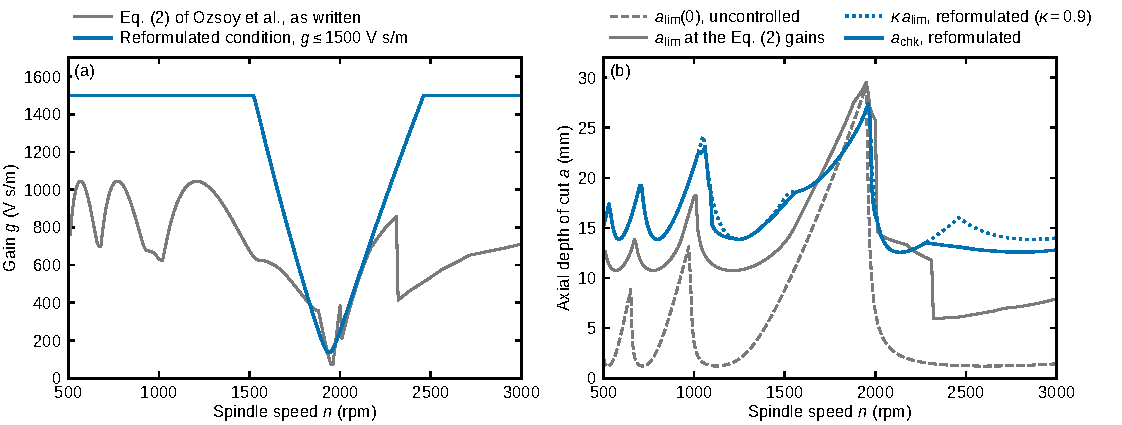
\includegraphics[width=\textwidth]{figures/fig02_feasibility.pdf}
  \caption{Gain scheduling under the two authority conditions over \SIrange{500}{3000}{\rpm}. (a)~Gain maps: the published condition, Eq.~\eqref{eq:pub}, reproduced with a step entry, the reformulated condition, Eq.~\eqref{eq:feas} with $\mathcal G=[0,1500]$, and the published map of \citet{ozsoy2026robust}. (b)~Depths: uncontrolled limit $a_{\lim}(0)$, $a_{\lim}$ at the gains of Eq.~\eqref{eq:pub}, $\kappa a_{\lim}$ and the checked depth $a_{\mathrm{chk}}$ of Eq.~\eqref{eq:achk} at the reformulated gains.}
  \label{fig:feas}
\end{figure}

\section{Saturation-induced finite-amplitude instability}\label{sec:bistability}

A step entry, by saturating the command, tips cuts that the linear analysis calls stable into chatter (Section~\ref{sec:feasibility}). This section measures how large a disturbance the settled cut tolerates under the DVF law of Eq.~\eqref{eq:dvf} with its hard clip, what happens beyond it, and how the tolerated disturbance depends on the residual authority. A cut is said to show \emph{finite-amplitude instability} when its forced orbit is linearly stable but a finite perturbation ends in chatter, and to be \emph{bistable} when, in addition, that chatter is a bounded attractor (Section~\ref{sec:bistab-attr}).

\subsection{Simulation protocols}\label{sec:bistab-prot}

All runs use the simulator of \ref{app:simulator}, the gains of Section~\ref{sec:feasibility} ($\mathcal G=[0,1500]$) and, unless stated otherwise, the clipped command. In the \emph{step entry} the full depth and immersion act from $t=0$, starting from rest with zero history. In the \emph{face entry} the tool advances into a workpiece face normal to the feed and reaches full engagement after 40 revolutions. In the \emph{feed ramp} the feed per tooth rises linearly from zero to $f_z$ over ten revolutions. The depth limit of an entry was found on a ladder of depths up to $1.05\alim$, refined by bisection (Supplementary Material), each run being judged over the 300 revolutions after the entry.
% src: src/tdsim.c (opt[1]-opt[3]: ramp_f, f0, edge), src/tdsim.py (entry_revs), src/c1_unsafe_zone.py (ENTRIES, LADDER), src/tdboundary.py (boundary, classify: rtol 3e-3, NREV 300); README §11.2

In the kick protocol the cut was settled by a face entry, and at revolution 100 a velocity increment $\Delta v$, the \emph{kick}, was added to $\dot x$ at one of 16 phases $\theta$ per tooth period; the 300 revolutions after it were classified. The \emph{critical kick} $\Delta v^*(\theta)$ is the smallest kick that ends in chatter; as the outcome is not monotone in $\Delta v$ (a large kick throws the tool out of the cut), it was found by an upward search up to \SI{3}{\metre\per\second} (Supplementary Material). The lower edge of the \emph{unsafe band}, in the sense of the unsafe zones of milling \citep{dombovari2015bistable,dombovari2019experimental}, was mapped every \SI{20}{\rpm} (126 speeds) as the smallest depth at which one of seven kicks from \SI{3}{\milli\metre\per\second} to \SI{3}{\metre\per\second} ends in chatter. The checks of these protocols asked for in the literature on bistable zones (kick timing, number of phases, window length, holes in the band) are collected in Section~\ref{sec:bistab-checks}.
% src: src/c1_unsafe_zone.py (KICK_REV = 100, WINDOW = 300, N_PHASE = 16, DV_GRID, N_BISECT = 6, BAND_STEP = 20, BAND_DV, BAND_PHASES = 2, BAND_BISECT = 6, _critical_kick, _band_low)

As a kick or an entry transient can throw the tool out of the cut for many passes, the chip is cut against the deepest earlier pass at the same angle [Eq.~\eqref{eq:surf}] \citep{tlusty1981basic}, a full memory without which clipped chatter can grow spuriously beyond \SI{1}{\centi\metre} (\ref{app:simulator}; Supplementary Material); only the off-axis runs of Section~\ref{sec:cert-c3} used the last four passes (\ref{app:lmi}). A run whose displacement exceeds \SI{1}{\centi\metre}, 200 feeds, is stopped and counted as chatter: such an excursion is a failure of the cut, whatever the model, far outside its validity, would do afterwards. Runs are classified by the criterion D1 of \ref{app:simulator}, which biases step-entry boundaries near $\alim$ high, by \SIrange{0.05}{1.5}{\percent} and by up to \SI{4.4}{\percent} near the forced resonance, but not kick-based limits or clipped limits well below $\alim$.
% src: README §11.2; verification/tdsim/check9_full_memory.json (bounded clipped chatter 0.43-0.59 mm with full memory and brute force; 1050 rpm, 0.9 a_lim diverges with both; nreg 4: 2 of 4 diverge, 0.554 vs 0.435 mm); src/tdboundary.py; verification/tdsim/check8_onset_long_runs.json (bias 0.05-1.47 %), check10_forced_resonance_long_runs.json (up to 4.4 %)

\subsection{The same cut, two outcomes}\label{sec:bistab-two}

At \SI{2500}{\rpm} with $g=1500$ ($\alim=\SI{17.24}{\milli\metre}$) and $a=\SI{15}{\milli\metre}$, the step entry ends in clipped chatter of about \SI{0.43}{\milli\metre}, whereas the face entry settles on the forced orbit with a command of about \SI{5}{\volt}. Figure~\ref{fig:two} shows the settled cut at $0.9\alim$, kicked just below and just above the critical kick of that phase, \SI{7.29}{\milli\metre\per\second}: after the smaller kick the motion returns to the forced orbit although the command still reaches the clip, after the larger one it grows into clipped chatter. The forced orbit and clipped chatter therefore coexist, and in this linear-force model, at kicks of this size, it is the saturation that makes them coexist: without the clip, chatter required kicks at least 50 times larger (Section~\ref{sec:bistab-basin}). The mechanism is a loss of effective gain (Section~\ref{sec:bistab-df}): once the chatter component, added to $b(t)$, reaches $\Vmax$, the clip passes on only part of the feedback, and the growing chatter saturates the command further.
% src: README §11.3; verification/tdsim/check9_full_memory.json (2500 rpm, 15 mm, step entry, full memory: max |x| = 0.435 mm); paper/figures/figure_numbers.json (fig03: 0.9 a_lim = 15.51 mm, kicks 7.0/7.6 mm/s at phase 0, critical kick 7.29 mm/s); results/c1_basin.npz (2500 rpm, 0.9 a_lim, clipped: phase 0 7.288 mm/s); closed form of Eq. (xp) gives b_max = 5.37 V at 15 mm (cross-check of README "about 5 V"); ratio 50: results/c1_basin.npz (smallest ratio of unclipped to clipped minimum kick, 52.1)

\begin{figure}[!tbp]
  \centering
  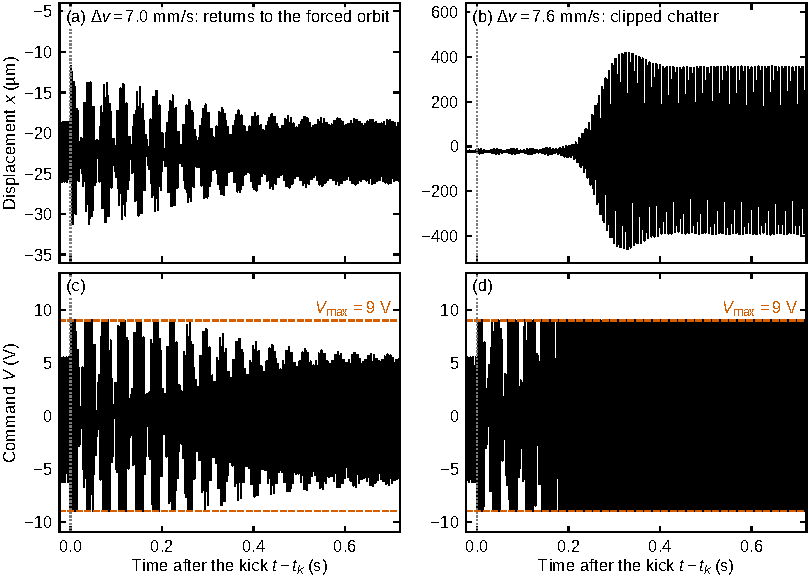
\includegraphics[width=\textwidth]{figures/fig03_two_outcomes.pdf}
  \caption{The same linearly stable cut (\SI{2500}{\rpm}, $g=\SI{1500}{\volt\second\per\metre}$, $a=0.9a_{\lim}=\SI{15.51}{\milli\metre}$, $\lvert V\rvert\le\SI{9}{\volt}$), settled by a face entry and kicked at the start of a tooth period, where the critical kick is \SI{7.29}{\milli\metre\per\second}. (a,\,c)~$\Delta v=\SI{7.0}{\milli\metre\per\second}$: the motion returns to the forced orbit. (b,\,d)~$\Delta v=\SI{7.6}{\milli\metre\per\second}$: it ends in clipped chatter. Top: displacement $x$; bottom: applied command $V$ and the clip $\pm V_{\max}$; dotted vertical line: the kick.}
  \label{fig:two}
\end{figure}
% src: paper/figures/figure_numbers.json (fig03), results/c1_basin.npz

\subsection{Entry limits over 251 speeds}\label{sec:bistab-map}

With the step entry the ratio of the clipped limit to $\alim$ has a median of 0.910 and a minimum of 0.736 (\SI{2460}{\rpm}), and it is below $0.97\alim$ at 157 of 251 speeds (Fig.~\ref{fig:map}). The face entry reaches at least $0.985\alim$ at every speed, and the feed ramp falls below $0.97\alim$ only at \SI{2000}{\rpm} ($0.957\alim$). Where the step entry binds, the better of the face entry and the feed ramp gains \SI{2.5}{\milli\metre} on average and up to \SI{4.7}{\milli\metre} (\SI{1980}{\rpm}). Without the clip the step-entry limit sits at the linear limit (median ratio 1.01; Supplementary Material).
% src: results/c1_map.npz, results/c1_summary.json (map: step_clip, edge_clip, feed_clip, step_free, soft_minus_step_mean_mm 2.51); results/c1_map.npz recomputed: largest gain of max(face, feed ramp) over the step entry where it binds 4.741 mm at 1980 rpm (19.02 vs 23.75 mm; 4.24 mm at 2500 rpm, 13.00 vs 17.25 mm); results/c1_map.npz recomputed: a_step_free/a_lim > 1.015 at 75 speeds (1.0165-1.050); a_edge_clip and a_feed_clip = 1.05 a_lim at 500, 540, 670, 720, 1000, 1080 rpm, a_step_clip at 500, 550, 670, 1000 rpm (seven speeds in all); at the other 245 speeds a_edge_clip mean 18.200 mm, a_lim mean 18.206 mm; results/feas_g1500.npz (at_bound: 157) vs results/c1_map.npz (a_step_clip < 0.97 a_lim: 157), 110 in common; verification/tdsim/check10_forced_resonance_long_runs.json

The lower edge of the unsafe band was found at 109 of the 126 speeds, at 0.21--$0.98\alim$ (median 0.46), and always above the uncontrolled limit, at no less than $1.08\alim(0)$. That the clip cannot create chatter below $\alim(0)$ is suggested by a describing-function argument, as the clip can only lower the effective gain, and is proved for the averaged model below a depth close to $\alim(0)$ in Section~\ref{sec:cert-global}. Above $\alim(0)$ a bounded basin is expected, since the uncontrolled cut is exponentially unstable there and no bounded input can stabilise it globally \citep{hu2001book}; what the simulations add is the size of the basin and its dependence on depth, speed and entry. No band was found at 17 speeds, most of them where the gain is small (Supplementary Material). The edge rests on kicks of up to \SI{3}{\metre\per\second}, far beyond the validity of the model; a scan of the depth confirms that the band has no holes (Section~\ref{sec:bistab-checks}). The step entry exposes only the top of the band, where the entry transient exceeds the basin.
% src: results/c1_band.npz, results/c1_summary.json (band: found 109/126, ratio 0.21/0.46/0.98, over_alim0_min 1.08, none_at_rpm, g_where_none); README §11.4

\begin{figure}[!tbp]
  \centering
  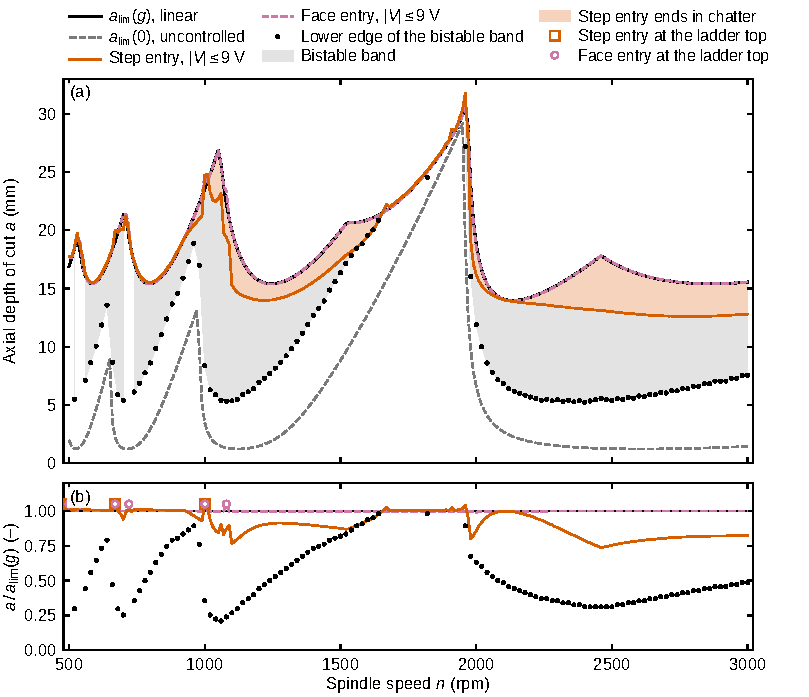
\includegraphics[width=\textwidth]{figures/fig04_entry_map.pdf}
  \caption{Depth limits over 251 speeds with the gains of Section~\ref{sec:feasibility} ($\mathcal G=[0,1500]$). (a)~Linear limit $a_{\lim}(g)$ and uncontrolled limit $a_{\lim}(0)$; time-domain limits with the \SI{9}{\volt} clip for the step entry and the face entry; lower edge of the unsafe band from kicks of \SI{3}{\milli\metre\per\second} to \SI{3}{\metre\per\second} on the settled cut (every \SI{20}{\rpm}). Shaded: the unsafe band, and the part of it in which the step entry ends in chatter. (b)~The same limits as fractions of $a_{\lim}(g)$; open markers: step-entry (squares) and face-entry (circles) limits at the top of the depth ladder, $1.05a_{\lim}$, above which they were not resolved.}
  \label{fig:map}
\end{figure}

\subsection{Basin of the forced orbit}\label{sec:bistab-basin}

Figure~\ref{fig:basin} and Table~\ref{tab:basin} give the critical kick at 1090, 1420, 2500 and \SI{2870}{\rpm} with $g=1500$, at twelve depths from 0.15 to $0.98\alim$ with the clip and at four without it. With the clip the basin is finite from 0.25--$0.80\alim$ onwards and narrows towards the limit. To give the kick a physical scale, its impulse $m\Delta v^*$ is compared with the mean cutting impulse of one tooth period,
\begin{equation}\label{eq:impulse}
  \bar F_yT,\qquad \bar F_y=\frac{N_t\,a\,f_z}{2\pi}\Bigl(\frac{\pi}{4}K_{tc}+\frac12K_{rc}\Bigr),
\end{equation}
where $\bar F_y$ is the mean static force normal to the feed. At $0.98\alim$ the critical kick of the worst phase carries \SIrange{2.4}{10.8}{\percent} of this impulse; as an equivalent displacement $\Delta v^*/\omega_n$ it is 2.9--\SI{13}{\micro\metre}, against a forced vibration of about \SI{4}{\micro\metre} amplitude at \SI{2500}{\rpm} and $0.9\alim$ (Fig.~\ref{fig:two}) and a feed of \SI{50}{\micro\metre}. Kicks of at most \SI{10}{\milli\metre\per\second} (\SI{12}{\micro\metre}) end in chatter only from 0.90--$0.95\alim$ upwards, if at all (Supplementary Material). Over the 16 phases the critical kick varies by at most \SI{24}{\percent}, so the basin is a property of the cut rather than of the timing of the disturbance.
% src: results/c1_basin.npz (dv, frac, vmax, tooth_impulse, mass), results/c1_summary.json (basin: first_finite_frac, impulse_098_pct, impulse_098_min_pct, phase_spread_098, phase_spread_max); src/c1_unsafe_zone.py (run_basin: tooth impulse); verification/paper/revision_runs.json (stored.kick_displacement_098: worst-phase dv at 0.98 a_lim 10.88, 5.04, 2.34, 8.12 mm/s = 13.4, 6.2, 2.9, 10.0 um at omega_n = 2 pi 129.3 rad/s, 1090/1420/2500/2870 rpm; recomputed from results/c1_basin.npz); results/c1_basin.npz recomputed: smallest depth with worst-phase dv <= 10 mm/s: 0.95, 0.90, 0.95 a_lim at 1420, 2500, 2870 rpm, none at 1090; <= 30 mm/s: 0.40, 0.80, 0.40, 0.50 a_lim at 1090, 1420, 2500, 2870 rpm; 10 mm/s / omega_n = 12.3 um; paper/figures/figure_numbers.json (fig03 orbit_x_um -26.0 to -18.6, i.e. 3.7 um amplitude)

\begin{table}[!tbp]
  \centering
  \caption{Critical kick $\Delta v^*$ of the clipped cut ($g=\SI{1500}{\volt\second\per\metre}$, $\lvert V\rvert\le\SI{9}{\volt}$): median over 16 phases and, in parentheses, the worst phase. The last column gives $m\Delta v^*$ as a percentage of the cutting impulse $\bar F_yT$ of Eq.~\eqref{eq:impulse}. Basin finite from: the smallest of the 12 depths at which some kick of at most \SI{3}{\metre\per\second} ends in chatter.}
  \label{tab:basin}
  \begin{tabular}{@{}rcccc@{}}
    \toprule
    Speed & Basin finite & \multicolumn{2}{c}{$\Delta v^*$ (\si{\milli\metre\per\second})} & $m\Delta v^*/(\bar F_yT)$ (\si{\percent})\\
    \cmidrule(lr){3-4}
    (rpm) & from $a/a_{\lim}$ & $a=0.9a_{\lim}$ & $a=0.98a_{\lim}$ & $a=0.98a_{\lim}$\\
    \midrule
    1090 & 0.25 & 15.3 (15.1) & 11.5 (10.9) & 4.3 (4.0)\\
    1420 & 0.80 & 13.7 (12.5) & 5.3 (5.0)   & 3.0 (2.9)\\
    2500 & 0.40 & 8.3 (7.2)   & 2.5 (2.3)   & 2.6 (2.4)\\
    2870 & 0.50 & 11.8 (11.5) & 8.7 (8.1)   & 11.5 (10.8)\\
    \bottomrule
  \end{tabular}
\end{table}
% src: results/c1_basin.npz; results/c1_summary.json (basin); README §11.5

Without the clip, no kick up to \SI{3}{\metre\per\second} ended in chatter at 13 of the 16 tested points; at the other three only kicks of 0.78--\SI{3}{\metre\per\second} in one phase did, the loss-of-contact bistability of milling without an actuator \citep{dombovari2015bistable}. In this linear-force model the clip thus shrinks the basin by a factor of 52--701 where the unclipped cut is itself bistable, and creates the bistability, on this range of kicks, at nine further points (Supplementary Material).
% src: results/c1_basin.npz (vmax = 0 rows; ratios of the smallest unclipped to the smallest clipped kick: 52.1, 275.7, 700.9; lower bounds 3 m/s / clipped minimum: 69.7-594.9); README §11.5

\subsection{What lies beyond the basin}\label{sec:bistab-attr}

The classifier shows that the basin is bounded, not where a trajectory that leaves it goes. At the 29 points of Table~\ref{tab:basin} where the basin is finite, the settled cut was therefore kicked at the worst phase with 2, 2.5 and 3 times the critical kick and followed for 2000 revolutions with the full surface memory. All 87 runs ended in bounded chatter whose statistics in the second and in the last quarter of the run agree (root mean square of $x$ and of $V$ within \SI{10}{\percent}, clipped fraction of the time within 0.05, chatter frequency within \SI{1}{\hertz}); none exceeded \SI{1}{\centi\metre} and none returned to the forced orbit. The chatter does not depend on the kick, its root mean square displacement differing by less than \SI{0.09}{\percent} between the three kicks. It keeps the command on the clip for 89--\SI{99}{\percent} of the time, at 133--\SI{153}{\hertz}, with a peak-to-peak displacement of 0.08--\SI{2.0}{\milli\metre}, far larger than the feed per tooth, so that the tool leaves the cut periodically, which bounds the amplitude \citep{tlusty1981basic}; at least \SI{98}{\percent} of its energy is not synchronous with the tooth passing. Continued to 4000 revolutions at the four points at $0.9\alim$, its root mean square and frequency change by less than \SI{0.13}{\percent} and \SI{0.003}{\hertz}. At these points the clipped cut is therefore bistable in the strict sense: the forced orbit coexists with a bounded, stationary chatter attractor (Fig.~\ref{fig:attr}).
% src: verification/paper/attractors_kick.json (summary: 29 points run, 87 runs, outcome_counts bounded_stationary 87; Q4 pp_x 0.081-1.993 mm, rms_V 8.67-8.98 V, clip_frac 0.891-0.992, f_chatter 132.7-153.1 Hz, nonsync_frac >= 0.978; max_rel_spread_rms_x_over_kicks <= 8.9e-4; long_runs at 0.9 a_lim: rel_change_rms_x <= 1.3e-3, change_f_chatter <= 2.0e-3 Hz)

Bifurcation-type diagrams against the depth place these attractors over the whole range (Fig.~\ref{fig:attr}a--d). At 28 depths from $\alim(0)$ to $1.05\,\alim$, the cut was started by a face entry, by the same with a kick of 0.03 or \SI{0.3}{\metre\per\second} at revolution 100, and by a step entry, and was run for 1600 revolutions. Every start ended either on the forced orbit or in bounded, stationary chatter; none exceeded \SI{1}{\centi\metre}. The chatter branch, reached from at least one start, begins at 0.25, 0.74, 0.31 and $0.44\,\alim$ at 1090, 1420, 2500 and \SI{2870}{\rpm} (its lower ends refined by bisection, consistent with the coarser depth grid of Table~\ref{tab:basin}) and coexists with the forced orbit up to the linear limit, one to two orders of magnitude larger than the forced vibration. Over these ranges the clipped cut is bistable. Once per tooth period the chatter traces a closed curve around the fixed point of the forced orbit (Fig.~\ref{fig:attr}e), and its spectrum is dominated by a component at \SI{134.6}{\hertz} with combination tones around the tooth-passing harmonics (Fig.~\ref{fig:attr}f): the chatter is quasi-periodic. Twin runs whose kicks or depths differ by a relative $10^{-9}$ stay within $5\times10^{-7}$ of its peak-to-peak amplitude after 1600--2000 revolutions at ten points, so it is regular, not chaotic. The amplitude settles within some tens of revolutions after the kick (Fig.~\ref{fig:attr}g).
% src: verification/paper/attractors_bifurcation.json/.npz (28 depths a_lim(0)-1.05 a_lim, ICs face, kick0.3, kick0.03, step, NREV 1600; states forced/chatter only, no diverged; refine_lo/hi: 5.23-5.25, 13.18-13.19, 5.36-5.38, 6.76-6.78 mm = 0.249/0.741/0.311/0.439 a_lim); paper/figures/figure_numbers.json (fig_attr: bifurcation, spectra_2500_09 peak 134.6 Hz); verification/paper/attractors_chaos.json (10 cases, verdict regular, sep_final_over_pp <= 4.9e-7)

Away from these four speeds the picture is not uniform. A spot check at 14 speeds where the band reaches deep cuts (a step entry and kicks of 0.03 and \SI{0.3}{\metre\per\second} at 0.9 and $0.98\,\alim$, 1600 revolutions) found bounded chatter at six of them, at \SI{980}{\rpm} two distinct chatter attractors at the same depth, and no chatter at the depths tested at three. At the other five, 700 and 1020--\SI{1060}{\rpm}, the runs exceeded the \SI{1}{\centi\metre} at which the simulator stops; with the stop raised to \SI{10}{\centi\metre}, all 21 returned to the forced orbit within 60 revolutions, after excursions of 12--\SI{30}{\milli\metre}. There the disturbed cut does not settle into chatter in the model but leaves the range of the model altogether, an excursion that no real cut would survive: the band map counts it as chatter, but it is not bistability.
% src: verification/paper/attractors_band_spot.json (summary: 14 speeds, 78 runs, state_counts forced 34, diverged (|x| > 1 cm) 21, chatter 23; speeds_with_divergence 700, 1020, 1040, 1050, 1060; speeds_bounded_only 960, 980, 1080, 1620, 1640, 1980; 980 rpm, 21.86 mm: chatter attractors of 0.084 mm at 168.5 Hz and 1.716 mm at 129.7 Hz; no chatter at the tested depths at 1000, 1820, 1960 rpm); verification/paper/attractors_abort.json (abort 0.1 m: 21/21 forced, max_x 12.5-30.3 mm, back on the forced orbit after 18-59 revolutions, D1 stable)

\begin{figure}[!tbp]
  \centering
  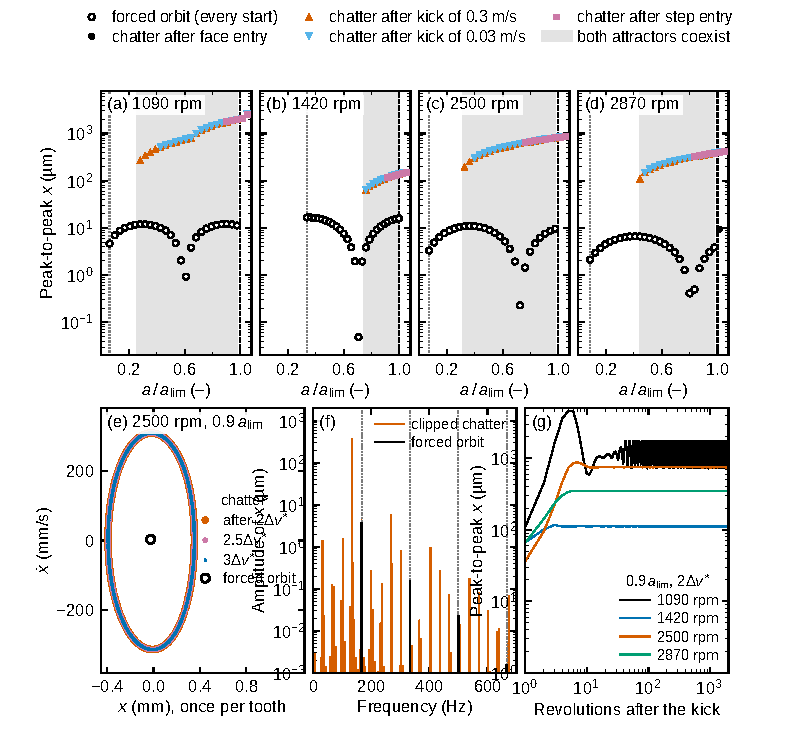
\includegraphics[width=\textwidth]{figures/fig_attractors.pdf}
  \caption{What lies beyond the basin ($g=\SI{1500}{\volt\second\per\metre}$, $\lvert V\rvert\le\SI{9}{\volt}$, full surface memory). (a)--(d)~Steady peak-to-peak displacement over the last 300 of 1600 revolutions against $a/\alim$, for four starts: open circles, the forced orbit, which every start reaches where it is the only attractor; filled markers, bounded chatter. Shaded: both attractors coexist; dotted: $\alim(0)$; dashed: $\alim$. (e)~Once-per-tooth samples of $(x,\dot x)$ of the last 500 tooth periods after kicks of 2, 2.5 and 3 times the critical kick, at \SI{2500}{\rpm} and $0.9\alim$: the three runs settle on the same closed curve around the forced orbit. (f)~Amplitude spectra of $x$ over 500 revolutions at the same point; dotted: tooth-passing harmonics. (g)~Peak-to-peak displacement per revolution after a kick of twice the critical kick at $0.9\alim$.}
  \label{fig:attr}
\end{figure}

\subsection{A describing-function prediction}\label{sec:bistab-df}

The size of the basin near the limit can be predicted with a dual-input describing function \citep{gelb1968describing}; actuator saturation in active vibration control of milling has also been modelled in the frequency domain by \citet{ozsoy2025frequency}, and whether that model already contains the forced command and a threshold amplitude, and so how far the estimate below goes beyond it, was not examined. Near the limit the deviation from the orbit is dominated by the chatter mode, and the unclipped command is $u=b(t)+A\sin\omega_ct$, with $A$ the amplitude of its chatter component and $\omega_c$ the chatter frequency. For $\omega_c$ incommensurate with $\omega_T$, the clip acts on the chatter component as the gain
\begin{equation}\label{eq:df}
  \mathcal N(A)=\lim_{\tau_a\to\infty}\frac{2}{A\tau_a}\int_0^{\tau_a}\operatorname{sat}_{V_{\max}}\bigl(b(t)+A\sin\omega_ct\bigr)\sin\omega_ct\,\mathrm dt\ \le 1,
\end{equation}
and the clipped loop thus behaves like DVF with the effective gain $\mathcal N(A)\,g$. A cut of depth $a<\alim(g)$ needs only the gain $g_e(a)$, the largest gain not above $g$ with $\alim(g_e)=a$, and chatter can be sustained once the gain of Eq.~\eqref{eq:df} falls below $g_e(a)/g$, i.e.\ above a critical amplitude $A^*(a)$. A kick $\Delta v$ excites the chatter mode with a velocity amplitude $p\,\Delta v$, where $p$ was fitted on the unclipped cut from the decay of its least-damped mode after a small kick (Supplementary Material). Hence
\begin{equation}\label{eq:dfbasin}
  \Delta v^*_{\mathrm{DF}}(a)=\frac{A^*(a)}{g\,p},\qquad
  \Delta v^*_{\mathrm{DF}}\;\to\;\frac{V_{\max}-b_{\max}}{g\,p}\quad\text{as }a\to a_{\lim},
\end{equation}
the limit holding because $g_e\to g$ and $\mathcal N(A)=1$ as long as $\bmax+A\le\Vmax$.
% src: src/c1_unsafe_zone.py (df_gain: 128 phases, b on 128 samples per tooth period; critical_amplitude; effective_gain_needed; _mode_factor: kick of 1 mm/s at phase 0, high-pass 40 Hz, fit of the slowest decaying mode)

Where $p$ could be fitted, from 0.7--$0.8\alim$ upwards, the simulated critical kick (median over the phases) is 0.61--1.13 times this estimate, and 0.88--1.13 times at 0.95 and $0.98\alim$ (Fig.~\ref{fig:basin}). Equation~\eqref{eq:dfbasin} predicts that the basin does not close at the limit but tends to a finite size, set by the voltage that the forced command leaves free; this is a prediction of the describing function, not a proven property of the basin at the limit itself. At $\alim$ the residual authority is $\Vmax-\bmax=3.9$, 1.7, 0.87 and \SI{4.7}{\volt} at 1090, 1420, 2500 and \SI{2870}{\rpm}, and at $0.999\alim$ the simulated critical kick is still 1.4--\SI{10.5}{\milli\metre\per\second} at the three speeds tested (Supplementary Material). The basin would close below $\alim$ only where $\bmax$ reached $\Vmax$; the authority condition of Section~\ref{sec:feasibility} keeps $\bmax\le\Vmax$ up to $\kappa\alim$, but with equality at some depth at the 94 speeds (1530--\SI{2460}{\rpm}) where the steady demand binds (Sections~\ref{sec:feas-res} and~\ref{sec:cert-c2}). This residual authority is fragile against persistent forcing that adds to $b$, such as runout (Section~\ref{sec:delayed-robust}). The estimate is cheap, but it rests on the filtering hypothesis and on the factor $p$, fitted at one kick phase and valid only near the limit; $A^*$ is the harmonic-balance amplitude of the unstable limit cycle that bounds the basin.
% src: results/c1_df.npz (A_dual at a = a_lim: 3.92, 1.66, 0.87, 4.69 V at 1090, 1420, 2500, 2870 rpm = V_max - b_max; the 1420 rpm value was 0.009 V before a round-off fix in c1_unsafe_zone.critical_amplitude, tests/test_c1_results.py), results/c1_basin.npz (p_mode finite at frac >= 0.7, at 1420 rpm >= 0.8), results/c1_summary.json (td_over_df 0.61-1.13); ratios at 0.95/0.98 recomputed with the c1_summary formula: 0.88-1.13; verification/tdsim/check11_kick_near_limit.json (1.405-1.467, 7.055-7.611, 9.150-10.533 mm/s); README §11.5; verification/paper/revision_runs.json (closed_form.runout_to_clip_g1500: 0.730, 3.09, 8.74 um at 2500, 2870, 1420 rpm; 1090 rpm below 9 V up to 10 um; worst command over 40 depths up to 0.9 a_lim and 8 runout phases, c4_robust.worst_orbit_command)

\begin{figure}[!tbp]
  \centering
  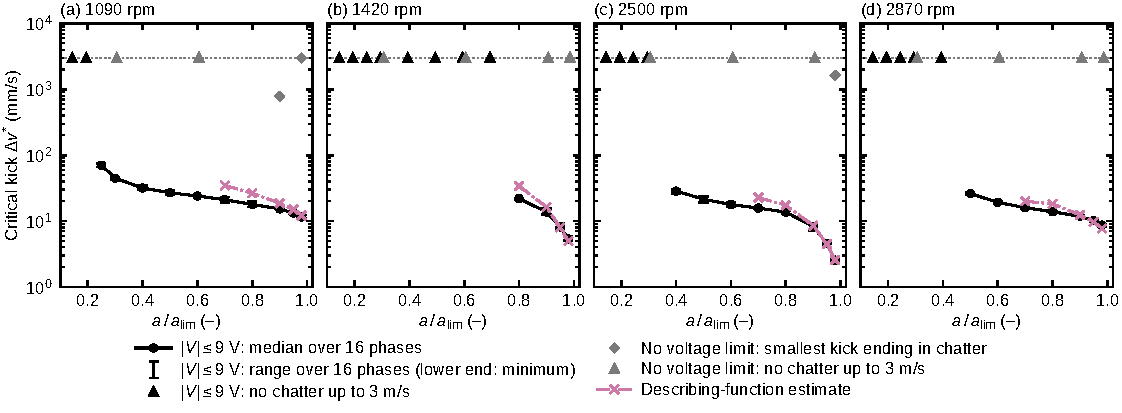
\includegraphics[width=\textwidth]{figures/fig05_basin.pdf}
  \caption{Critical kick $\Delta v^*$ against $a/a_{\lim}$ at (a)~1090, (b)~1420, (c)~2500 and (d)~\SI{2870}{\rpm} ($g=\SI{1500}{\volt\second\per\metre}$). With the \SI{9}{\volt} clip: median over 16 phases (circles) and range over the phases (bars; lower end: worst phase); black triangles: no chatter for any kick up to \SI{3}{\metre\per\second}. Without the clip: smallest kick that ends in chatter (diamonds) or no chatter up to \SI{3}{\metre\per\second} (grey triangles). Crosses: describing-function estimate, Eq.~\eqref{eq:dfbasin}. Right axis of (d): the kick as an equivalent displacement $\Delta v^*/\omega_n$.}
  \label{fig:basin}
\end{figure}

\subsection{Depth limit against the gain}\label{sec:bistab-gain}

At 1090 and \SI{2500}{\rpm} the entry limits were also computed for $g$ up to \SI{3000}{\volt\second\per\metre}. With the step entry the clipped limit nearly stops rising above about \SIrange{1500}{1650}{\volt\second\per\metre}, at about 19.8 and \SI{13.2}{\milli\metre}, while $\alim$ reaches 41.8 and \SI{40.0}{\milli\metre} at $g=3000$; the face entry follows $\alim$ until the forced command itself exceeds the clip (Supplementary Material). At large gains the depth at these two speeds is thus limited by the basin, which the entry transient exceeds, and not by the gain. Below the plateau the clipped step-entry limit rises with the gain, at \SI{2500}{\rpm} from \SI{6.4}{\milli\metre} at the reproduced gain of Eq.~\eqref{eq:pub} (\SI{536}{\volt\second\per\metre}), so in this model clipping a larger gain does not weaken DVF; the clipped-DVF comparison of \citet[Table~3]{ozsoy2026robust}, whose clipped gain is set by a tuning rule, was not reproduced.
% src: results/c1_gainplane.npz (a_step_clip, a_edge_clip, a_lim, orbit_peak_V), results/c1_summary.json (gainplane: step_clip_plateau_mm 19.78 and 13.19, a_lim_at_3000 41.82 and 40.03, orbit_saturates_from_g 3000 and 1650); README §11.6, §13.6; results/table3_main.csv (2500 rpm: a_prop_td 6.37 mm at the reproduced gain 535.6 V s/m; a_clip3000_td 13.23 mm), table3_clip_gain_sweep.csv; a_step_clip of c1_gainplane.npz rises monotonically with g at both speeds; README §5.5

\subsection{Checks of the protocols}\label{sec:bistab-checks}

\NEWCHECKS

\section{Certified basins of attraction}\label{sec:certificates}

The critical kick $\Delta v^*$ of Section~\ref{sec:bistability} samples the basin of the forced orbit in one direction of the state space, at 16 phases and on a grid of kick sizes; it cannot exclude chatter after a disturbance in another direction. This section proves inner estimates of the basin instead: ellipsoids of deviations from the forced orbit from which every trajectory returns to the orbit despite the clip. Unlike regional guarantees for chatter controllers designed with input constraints \citep{zhang2015ellipsoid,wu2016adaptive}, the DVF law is fixed and analysed, the clip acts on the voltage, and the dead zone is taken around the forced command $b(t)$, so that the authority spent on the forced orbit enters the certificate. Certificate C2 uses the averaged model and C3 the time-periodic model; both are checked independently of the solver and compared with the simulator of \ref{app:simulator}.

\subsection{Deviation dynamics and what is proved}\label{sec:cert-model}

Let $x_p(t)$ be the $T$-periodic forced orbit of Section~\ref{sec:model-orbit} and $b(t)=-g\dot x_p(t)$ its command, with $\bmax<\Vmax$ so that the clip is inactive on the orbit. Since $x_p(t)-x_p(t-T)=0$, the regenerative force vanishes on the orbit, and the deviation $\tilde x=x-x_p$ obeys
\begin{equation}\label{eq:dev}
\begin{aligned}
&m\ddot{\tilde x}+c\dot{\tilde x}+k\tilde x=aH(t)\,\big[\tilde x(t)-\tilde x(t-T)\big]+K_a\ddot{\tilde q},\\
&\ddot{\tilde q}+2\zeta_a\omega_a\dot{\tilde q}+\omega_a^2\tilde q=\sat_{\Vmax}\!\big(b(t)-g\dot{\tilde x}\big)-b(t),
\end{aligned}
\end{equation}
where $\tilde q$ is the deviation of the actuator coordinate of Eq.~\eqref{eq:eom} and $aH(t)$ is the $T$-periodic coefficient of the regenerative force, Eq.~\eqref{eq:aHt}. C2 replaces it by its mean $\overline{aH}$, Eq.~\eqref{eq:aHmean}, as in the zero-order approximation \citep{altintas1995analytical}; C3 keeps $aH(t)$.

The history $\tilde x(t+\vartheta)$, $\vartheta\in[-T,0]$, is represented by its values at the Chebyshev nodes $\vartheta_j=-\tfrac T2\big(1-\cos\tfrac{\pi j}{N}\big)$, $j=1,\dots,N$, and its transport equation is collocated with the Chebyshev differentiation matrix \citep{breda2005pseudospectral,breda2015book}. With $\xi=\big[\tilde x,\ \dot{\tilde x},\ \tilde q,\ \dot{\tilde q},\ \tilde x(t+\vartheta_1),\dots,\tilde x(t+\vartheta_N)\big]^\top\in\mathbb R^{4+N}$,
\begin{equation}\label{eq:coll}
\dot\xi=\mathcal A(t)\,\xi-B\,\psi(K\xi,t),\qquad \mathcal A(t)=A_0+BK+aH(t)\,E,
\end{equation}
with $K=-g\,e_2^\top$, $E=\big(e_2e_1^\top-e_2e_{4+N}^\top\big)/m$, $e_i$ the unit vectors, and $A_0$, $B$ in Eq.~\eqref{eq:app-A0}. The linear DVF loop stays in $\mathcal A$; the clip enters only through the dead zone
\begin{equation}\label{eq:deadzone}
\psi(w,t)=w-\sat_{\Vmax}\!\big(b(t)+w\big)+b(t),
\end{equation}
which vanishes for $-\Vmax-b(t)\le w\le\Vmax-b(t)$; unlike the dead zone of a fixed saturation, it moves with the forced command and is asymmetric whenever $b(t)\neq0$. The number of nodes is $N=16+4\lceil T\omega_n/2\pi\rceil$, 20--32 over 500--\SI{3000}{\rpm} (24 at 1090 and \SI{1420}{\rpm}, 20 at 2500 and \SI{2870}{\rpm}). For the averaged model the rightmost eigenvalues of Eq.~\eqref{eq:coll} agree with those of the delay equation to $3\times10^{-8}$, and the collocated model loses stability at $\alim$.
% src: README §12.2; src/c2_certificate.py (model, nodes_for, history_nodes); src/c3_periodic.py (model); tests/test_c2_certificate.py (crossing at a_lim)

The certificates are therefore theorems about Eq.~\eqref{eq:coll}, the $N$-node collocation of the averaged (C2) or the time-periodic (C3) model; they are not theorems about the delay equation, which would require a Lyapunov--Krasovskii functional \citep{seuret2014bessel}, nor about the simulator. Two effects of the simulator lie outside Eq.~\eqref{eq:coll}: the chip vanishing near the exit angle and, for C2, the variation of $aH(t)$, about $\pm12\,\%$ around its mean near the limit at half immersion and more at shallow depths.
% src: README §12.2, §14.10

\subsection{Sector condition and LMI conditions}\label{sec:cert-lmi}

Here $\bmax$ denotes an upper bound of $\max_t\lvert b(t)\rvert$, not a sampled peak, and $u_0=\Vmax-\bmax>0$. For all $t$, $w$ and $v$,
\begin{equation}\label{eq:sector}
\lvert w-v\rvert\le u_0\quad\Longrightarrow\quad\psi(w,t)\,\big[\psi(w,t)-v\big]\le0 .
\end{equation}
If $w>\Vmax-b(t)$, then $\psi=w-\Vmax+b(t)>0$ and $v\ge w-u_0\ge\psi$ since $b(t)\le\bmax$; the case $w<-\Vmax-b(t)$ is symmetric, and $\psi=0$ otherwise. Eq.~\eqref{eq:sector} is the generalised sector condition of \citet{gomesdasilva2005antiwindup} for the moving dead zone, with the level $u_0=\SI{9}{\volt}-\bmax$: the authority spent on the forced orbit is removed from the level. With $v=\Gamma\xi$ for a free row vector $\Gamma$, $\mathcal V(\xi)=\xi^\top P\xi$, $W=P^{-1}$, $Y=\Gamma W$ and a scalar multiplier $S>0$, the S-procedure \citep{tarbouriech2011book} gives, for the averaged model ($\mathcal A$ constant),
\begin{gather}
\begin{bmatrix}-(\mathcal AW+W\mathcal A^\top)-2\lambda W & BS-Y^\top\\ SB^\top-Y & 2S\end{bmatrix}\succ0, \label{eq:lmi-dec}\\
\begin{bmatrix}W & WK^\top-Y^\top\\ KW-Y & u_0^2\end{bmatrix}\succeq0, \label{eq:lmi-incl}\\
\begin{bmatrix}W & Wc^\top\\ cW & (\delta f_z)^2\end{bmatrix}\succeq0,\qquad c=e_1^\top-e_{4+N}^\top,\quad \delta=0.5, \label{eq:lmi-valid}\\
\begin{bmatrix}1 & \beta e^\top\\ \beta e & W\end{bmatrix}\succeq0. \label{eq:lmi-size}
\end{gather}
Inequality~\eqref{eq:lmi-incl} places $\mathcal E(P)$ in the region $\lvert(K-\Gamma)\xi\rvert\le u_0$, where Eq.~\eqref{eq:sector} holds with $w=K\xi$, and Eq.~\eqref{eq:lmi-dec} with $\lambda=0$ then makes $\mathcal V$ decrease strictly along every trajectory in $\mathcal E(P)$, at every $t$, because Eq.~\eqref{eq:sector} holds uniformly in time. $\mathcal E(P)$ is thus forward invariant, and every deviation in it returns to the forced orbit, whatever its phase. The margin $\lambda>0$ is asked of the solver only; the independent check tests $\lambda=0$, so no decay rate is claimed.

Inequality~\eqref{eq:lmi-valid} keeps $\mathcal E(P)$, and with it the whole trajectory, inside $\lvert x-x(t-T)\rvert\le0.5f_z$ (as $x_p$ is $T$-periodic, $\tilde x-\tilde x(t-T)=x-x(t-T)$). Without it, the ellipsoid at \SI{2500}{\rpm} and $0.7\alim$ contained states whose past was displaced by 7--12$f_z$, the tool being entirely out of the cut; they return in the linear model, but 32 of the 72 off-axis runs at that point (Section~\ref{sec:cert-c2}) ended in chatter, against 0 of 72 with the bound, whose cost along the kick direction is 0--16\,\%. The bound excludes only gross loss of contact: the chip can still vanish near the exit angle inside it. The value $\delta=0.5$ is a choice; $\delta=1$ raises the certificates by 0--15\,\%.
% src: README §12.2, §12.4, §12.7

The size $\beta$ in Eq.~\eqref{eq:lmi-size} is maximised along two directions. For $e=e_2$, a velocity kick at any phase moves the state to $\Delta v\,e_2$, since displacement and history are continuous, so $\beta$ is a certified kick in m/s. For $e=-\xi_p(0)$, minus the orbit state at $t=0$ with its history, $\beta$ is dimensionless: the cut that enters at rest on a fresh surface starts at $-\xi_p(0)$, so $\beta\ge1$ certifies the step entry at the entry phase of the simulator (tooth angle 0 at $t=0$), and only at that phase.

In C2, $\bmax$ was computed from samples of the orbit truncated at 40 harmonics, whose slice-force coefficients came from a discrete Fourier transform (\ref{app:lmi}). The closed-form bound of C3 is higher by 0.4--\SI{2.1}{\milli\volt} at the 48 validation points and by 0.1--\SI{3.3}{\milli\volt} on the surface grid. As all LMIs are homogeneous in $(W,Y,S)$, a certificate at the level $u_0$ remains valid at $u_0-d$ after scaling $(W,Y,S)$ by $\big((u_0-d)/u_0\big)^2$, which scales its size by $(u_0-d)/u_0$: by 0.997--1.000 at the 48 points and by down to 0.86 on the surface, where the margin almost vanishes. All C2 results below are corrected in this way.
% src: README §12.2, §14.9; results/c3_summary.json (errata: extra_mV 0.414-2.079 and 0.131-3.275, size_factor 0.9972-0.99995 and 0.858-1); src/c3_summary.py (margin_errata)

\subsection{Solution and independent check}\label{sec:cert-check}

The LMIs were assembled as sparse conic programs for the interior-point solver Clarabel \citep{goulart2024clarabel}, which stops short of the optimum on these problems. Each problem was solved three times: in coordinates scaled by the peak response of each state to a \SI{1}{\milli\metre\per\second} kick, then twice in coordinates whitened by the previous $W$ (re-centring). Every candidate $(W,Y,S)$ was checked independently of the solver: (i) $W\succ0$ with a condition number below $10^{10}$; (ii) the smallest eigenvalue of the matrix of Eq.~\eqref{eq:lmi-dec} at $\lambda=0$ above a round-off bound; (iii) the inclusion~\eqref{eq:lmi-incl} and the validity bound~\eqref{eq:lmi-valid}, evaluated through a Cholesky factor of $W$, an exceeded bound being repaired by scaling $(W,Y,S)$ down, which preserves (ii) by homogeneity; (iv) the size $\beta=(e^\top W^{-1}e)^{-1/2}$ from the same factor. The largest candidate that passed was kept, and the smaller of its checked size and the solver's $\beta$ is reported (settings in \ref{app:lmi}).
% src: src/c2_certificate.py (scaling, lmi, check, certify); README §12.3

\subsection{Extension to the time-periodic model}\label{sec:cert-periodic}

C3 keeps the periodic coefficient $aH(t)$ of Eq.~\eqref{eq:aHt}, with the integral over the depth evaluated in closed form. The forced orbit is that of C2, since regeneration vanishes on every $T$-periodic motion. At \SI{2500}{\rpm}, $aH(t)$ spans 0.89--1.08 times its mean at $0.9\alim$ and 0.36--1.42 times at $0.15\alim$, and the forced command $\lvert b(t)\rvert$ ranges over the period from nearly zero to \SI{7.9}{\volt} at $0.98\alim$, whereas C2 uses only its peak.
% src: README §14.1; src/c3_periodic.py (aH, orbit); ranges re-evaluated in closed form with c3_periodic.aH/orbit (0.886-1.079, 0.358-1.420; |b| 0.031-7.870 V)

The tooth period is divided into $M=16$ segments of length $\tau=T/M$, with nodes $t_k=k\tau$. On segment $k$, with $s=(t-t_k)/\tau\in[0,1]$,
\begin{equation}\label{eq:Wt}
W(t)=(1-s)W_k+sW_{k+1},\qquad Y(t)=(1-s)Y_k+sY_{k+1},\qquad S(t)=S_k,
\end{equation}
with $W_M=W_0$ and $Y_M=Y_0$, so that $\mathcal V(t,\xi)=\xi^\top W(t)^{-1}\xi$ is continuous and $T$-periodic. As $\mathrm d(W^{-1})/\mathrm dt=-W^{-1}\dot WW^{-1}$, the decrease condition becomes
\begin{equation}\label{eq:lmi-per}
\begin{bmatrix}\dot W_k-\mathcal A(t)W(t)-W(t)\mathcal A(t)^\top-2\lambda W(t) & BS_k-Y(t)^\top\\ S_kB^\top-Y(t) & 2S_k\end{bmatrix}\succ0,
\end{equation}
with $\dot W_k=(W_{k+1}-W_k)/\tau$, required at every $t$ of the segment. On each segment the coefficient is enclosed as $aH(t)=h_k+\ell_ks+r$, $\lvert r\rvert\le\varepsilon_k$: a least-squares line through 2048 samples and a residual bound widened by the variation possible between samples. $\mathcal A(t)W(t)$ then contains $s$, $s^2$ and $rs$, so that Eq.~\eqref{eq:lmi-per} is affine in $(s,\sigma)$, $\sigma=s^2$, for fixed $r$ and affine in $r$ for fixed $(s,\sigma)$. Since $(s,s^2)$ lies in the triangle with vertices $(0,0)$, $(\tfrac12,0)$ and $(1,1)$, the matrix at any time of the segment is a convex combination of its values at these three points combined with $r=\pm\varepsilon_k$, and positivity at the six vertices gives Eq.~\eqref{eq:lmi-per} on the whole segment.

The sector condition holds pointwise in time, so segment $k$ uses its own level $u_{0,k}=\Vmax-\max_{t_k\le t\le t_{k+1}}\lvert b(t)\rvert$ rather than $\Vmax-\bmax$. Inequalities~\eqref{eq:lmi-incl}--\eqref{eq:lmi-size}, written with $W(t)$, $Y(t)$ and $u_{0,k}$, are affine in $s$ and are imposed at both nodes of each segment. The tube $\{(t,\xi):\xi^\top W(t)^{-1}\xi\le1\}$ is then forward invariant and $\mathcal V$ decreases strictly in it: a deviation in $\mathcal E\big(W(t_0)^{-1}\big)$ at the phase $t_0$ returns to the orbit. As Eq.~\eqref{eq:lmi-size} is affine in $W$, a size that holds at both nodes of a segment holds between them; the certified kick valid at every phase is thus the smallest nodal size, and the sizes at the 16 kick phases of Section~\ref{sec:bistability} follow from $W(t)$ by interpolation. The tools are established, from piecewise-linear or clock-dependent time-varying Lyapunov matrices for switched, impulsive and periodic systems \citep{allerhand2011robust,briat2013clock,li2015periodic} to regions of attraction of saturated periodic systems \citep{zhou2011periodic,yang2015periodic,sakthivel2022jdsmc} and the control of periodic piecewise vibration systems with actuator saturation \citep{li2017hinfinity}, and \citet{cao2020switched} used a piecewise Lyapunov function, without a region of attraction, for active chatter control on a switched periodic milling model; what is new here is the application. The first solve starts in the coordinates of the C2 certificate, and every candidate is checked at all $6\times16$ vertices and all nodes (\ref{app:lmi}).
% src: README §14.2, §14.3, §14.9; src/c3_periodic.py (enclosure, corners, orbit, lmi, check, certify)

\subsection{Results on the averaged model (C2)}\label{sec:cert-c2}

C2 was computed at the 48 clipped points of Section~\ref{sec:bistability} (1090, 1420, 2500 and \SI{2870}{\rpm}; 12 depths from 0.15 to $0.98\alim$; $g=\SI{1500}{\volt\second\per\metre}$; Fig.~\ref{fig:cert}, Table~\ref{tab:cert}). All 48 certificates passed the check, with certified kicks of 0.96--\SI{12.9}{\milli\metre\per\second}. Each lies below the critical kick of its own model (the averaged collocated model with the true dead zone, minimum over four phases) at all 44 points where that kick is finite, and below $\Delta v^*$ (minimum over 16 phases) at all 29 points where $\Delta v^*$ is finite. $\Delta v^*/\beta$ is 1.48--27.6, largest at \SI{2500}{\rpm} and $0.4\alim$ ($\beta=\SI{0.96}{\milli\metre\per\second}$), and 1.48--3.26 (median 2.34) from $0.7\alim$ upwards. The averaged model is slightly more fragile than the simulated cut (critical kick 0.62--0.99 times $\Delta v^*$, median 0.92), so the gap lies mainly between the certificate and its own model.
% src: README §12.4; results/c2_validate.npz, c2_summary.json (validate), c3_summary.json (errata.c2_validate: 1.48-27.59, median 2.34 from 0.7 a_lim)

\begin{figure}[!tbp]
\centering
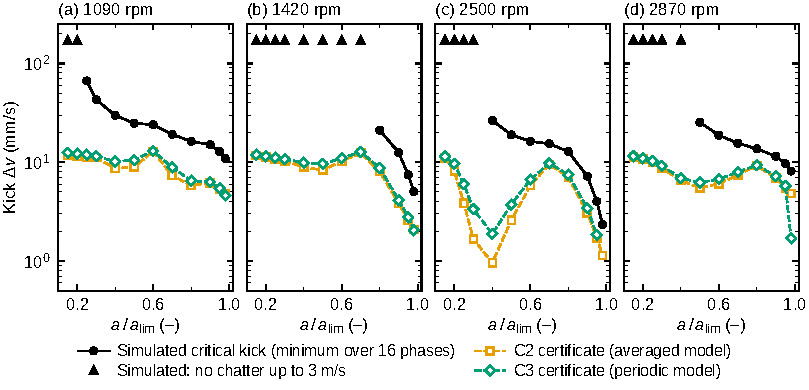
\includegraphics[width=\textwidth]{figures/fig06_certificates.pdf}
\caption{Certified kick on the averaged model (C2, squares; command bound corrected as in Section~\ref{sec:cert-lmi}) and on the periodic model (C3, diamonds; valid at every phase) against the simulated critical kick $\Delta v^*$ (circles; minimum over 16 phases), at (a) 1090, (b) 1420, (c) 2500 and (d) \SI{2870}{\rpm}, $g=\SI{1500}{\volt\second\per\metre}$, $\Vmax=\SI{9}{\volt}$. Triangles: no chatter for any kick up to \SI{3}{\metre\per\second}. C3 is missing at \SI{2500}{\rpm} and $0.98\alim$, where no candidate passed the check. Wherever $\Delta v^*$ is finite, both certificates lie below it.}
\label{fig:cert}
\end{figure}

\begin{table}[!tbp]
\centering
\caption{Validation of the certificates at the 48 clipped points of Section~\ref{sec:bistability} (four speeds, 12 depths from 0.15 to $0.98\alim$, $g=\SI{1500}{\volt\second\per\metre}$). $\Delta v^*$: simulated critical kick; C2 corrected for the command bound.}
\label{tab:cert}
\small
\begin{tabular}{@{}>{\raggedright\arraybackslash}p{0.36\textwidth}>{\raggedright\arraybackslash}p{0.27\textwidth}>{\raggedright\arraybackslash}p{0.27\textwidth}@{}}
\toprule
 & C2 (averaged model) & C3 (periodic model, $M=16$)\\
\midrule
Certificates that passed the check & 48/48 & 47/48\\
Certified kick $\beta$ (\si{\milli\metre\per\second}) & 0.96--12.9 & 1.70--13.0\\
$\beta$ below the model's critical kick & 44/44 (minimum over 4 phases) & 688/688 (per phase, 43 points)\\
$\beta$ below $\Delta v^*$ & 29/29 (minimum over 16 phases) & 448/448 (per phase, 28 points)\\
$\Delta v^*/\beta$, all points & 1.48--27.6 & 1.46--14.0\\
$\Delta v^*/\beta$ from $0.7\alim$ (median) & 1.48--3.26 (2.34) & 1.46--4.78 (2.27)\\
Model critical kick$/\Delta v^*$ (median) & 0.62--0.99 (0.92) & 0.61--0.98 (0.90)\\
Off-axis runs ending in chatter & 0/3456 & 0/3384\\
Sampled check, largest $\mathcal V$ & 0.998 (start value) & 0.997 (after the first step)\\
C3/C2 (median) & -- & 0.35--2.01 (1.064)\\
\bottomrule
\end{tabular}
\end{table}
% src: results/c2_summary.json, c3_summary.json (basin: cert_mm_s, phase_cert_below_model/td, td_over_cert, td_over_cert_from_07, model_over_td, offaxis, proof_vmax, c3_over_c2; errata.c2_validate); results/c2_validate.npz (C2 beta corrected 0.958-12.889 mm/s, model/TD 0.620-0.989)

A kick probes one of $4+N$ directions. Boundary points of $\mathcal E(P)$ in 18 directions (both signs of the points that maximise $\tilde x$, $\dot{\tilde x}$, $\tilde q$, $\dot{\tilde q}$, $\tilde x(t-T)$ and $\tilde x-\tilde x(t-T)$, and six random points) were therefore applied in the simulator as full-state deviations at four phases, with the kick protocol of Section~\ref{sec:bistability}; none of the 3456 runs ended in chatter. In addition, 48 trajectories of the collocated model with the true dead zone, started at 0.999 of the boundary in random directions and phases, never exceeded the initial $\mathcal V=0.998$. This sampled test is only a consistency check, since ellipsoids 2.5--3 times too large also pass it; the guarantee rests on the independent check.
% src: README §12.4; src/c2_certificate.py (boundary_directions, deviation_to_pert, td_offaxis, proof_check); results/c2_validate.npz (offaxis 0/3456, proof_vmax 0.998001)

The step entry is certified only at $0.3\alim$ at 1090, 1420 and \SI{2870}{\rpm} ($\beta=1.48$, 1.61 and 1.04) and never at \SI{2500}{\rpm} (at most 0.65, at $0.7\alim$), always below the simulated step-entry limits of 0.90, 0.89, 0.75 and $0.82\alim$ (Fig.~\ref{fig:surf}b--e). At 1090 and \SI{2870}{\rpm}, $0.3\alim$ is well above the uncontrolled limit, so the result is not trivial, but no productive depth is certified: at 0.5--$0.9\alim$, $\beta=0.16$--0.72. The certificate also depends on the entry phase. Applied at 64 entry phases at $0.3\alim$, it gives $\beta\ge1$ at only 24 phases at \SI{1420}{\rpm} (minimum 0.49) and 27 at \SI{1090}{\rpm}; certificates maximised for the worst phase reach 0.78 and 0.80, and only at \SI{2870}{\rpm} is the worst phase certified ($\beta=1.02$).
% src: README §12.5; results/c2_step.npz, c2_summary.json (step: td_step_limit_frac 0.895/0.893/0.754/0.821), c3_summary.json (errata.c2_step: 1.48/1.61/1.04 corrected); a_lim(0) recomputed with zoa.a_lim (1.26 and 1.32 mm against 6.30 and 4.62 mm); 64-phase and worst-phase values: README §12.5 only (not stored)

Over the gain map of Section~\ref{sec:feasibility}, at 42 speeds from 500 to \SI{2960}{\rpm} and seven depths from 0.5 to $0.98\alim$, 287 of 294 points were certified and checked (Fig.~\ref{fig:surf}a); at $0.9\alim$ the certified kick is 0--\SI{16}{\milli\metre\per\second}, with a median of \SI{6.6}{\milli\metre\per\second}. The other seven points lie at 1520--\SI{2000}{\rpm}, where the gain of the map sits at the authority limit: at three the forced orbit itself saturates ($u_0\le0$), and at four no candidate passed the check, with $u_0=0.04$--\SI{0.38}{\volt}, a numerical limit rather than a property of the cut. At 2060--\SI{2660}{\rpm} the forced orbit leaves little margin at shallow depths, and a kick of \SI{4}{\milli\metre\per\second} is not certified even at $0.5\alim$.
% src: README §12.6; results/c2_surface.npz (cert, u0, msg: failures at 1520/0.95, 1520/0.98, 1580/0.90, 1580/0.95, 1760/0.80, 1880/0.70, 2000/0.98), c2_summary.json (surface), c3_summary.json (errata.c2_surface: kick at 0.9 a_lim unchanged, 0-16.02, median 6.58)

\begin{figure}[!tbp]
\centering
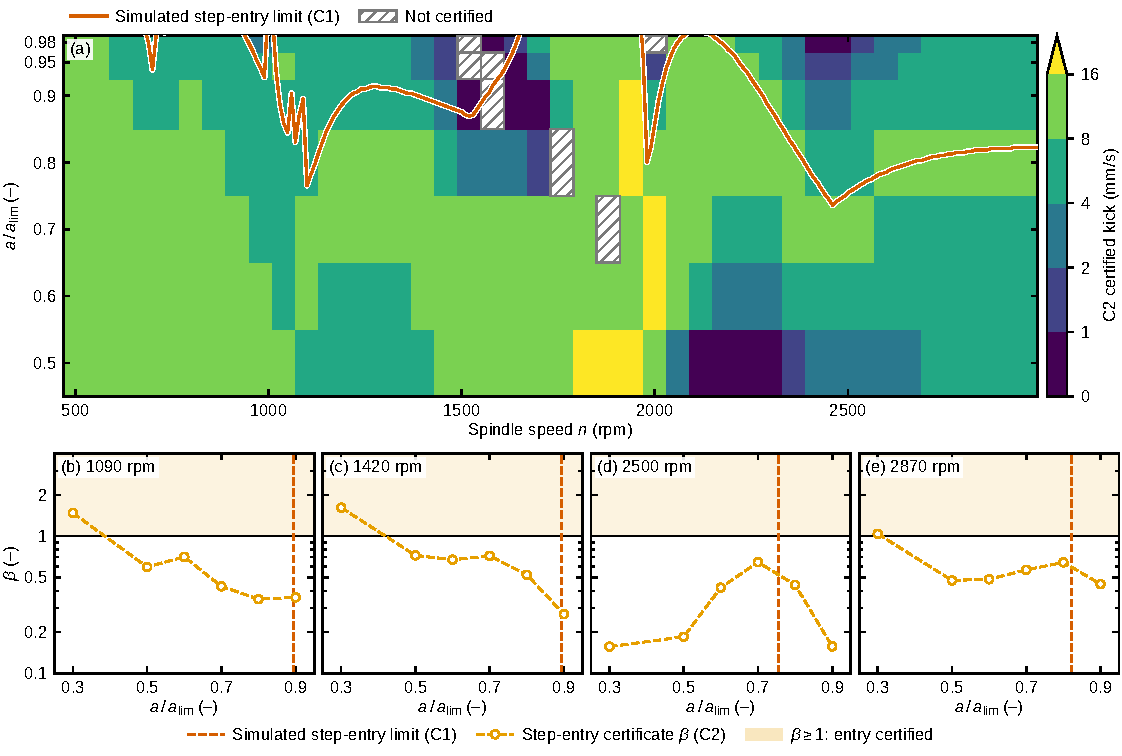
\includegraphics[width=\textwidth]{figures/fig07_certified_surface.pdf}
\caption{(a) Certified kick of the averaged model (C2) over spindle speed and depth on the gain map of Section~\ref{sec:feasibility}: 42 speeds, seven depths from 0.5 to $0.98\alim$; hatched: not certified (7 of 294 points); line: simulated step-entry limit of Section~\ref{sec:bistability}. (b)--(e) Step-entry certificate $\beta$ at the four speeds of Fig.~\ref{fig:cert}; $\beta\ge1$ (shaded) certifies the entry at rest on a fresh surface at the entry phase of the simulator; dashed: simulated step-entry limit. Command bound corrected as in Section~\ref{sec:cert-lmi}.}
\label{fig:surf}
\end{figure}

\subsection{Results on the periodic model (C3) and comparison with C2}\label{sec:cert-c3}

For the linear limit of this cutter averaging is nearly exact: on the gain map (126 speeds), the Floquet limit of the periodic collocated model is 0.99999--1.0011 times the averaged limit at half immersion and 0.99999--1.0028 times at the radial immersion $a_e/D=0.1$, never below it by more than $10^{-5}$ and without flip lobes (\ref{app:lmi}). The limits, 14--\SI{30}{\milli\metre} at half immersion and 30--\SI{65}{\milli\metre} at $a_e/D=0.1$, span one to five axial pitches $p_a$, over which the helix cancels most of the variation of $aH(t)$ \citep{insperger2006helix,zatarain2006helix}.
% src: README §14.4; results/c3_floquet.npz, c3_summary.json (floquet: 1.0000-1.0011 and 1.0000-1.0028, below_zoa 0, flip 0)

At the 48 points, 47 C3 certificates passed the check; at \SI{2500}{\rpm} and $0.98\alim$ none did (Table~\ref{tab:cert}). The ratio C3/C2 is 0.35--2.01 (median 1.064), and C3 exceeds C2 at 44 of the 47 points. The largest gains, 1.44--2.01, occur at \SI{2500}{\rpm} and 0.25--$0.5\alim$, where the worst segment leaves a margin of only 0.45--\SI{1.5}{\volt} and C2 is small (0.96--\SI{3.86}{\milli\metre\per\second}); at the other 40 points below $0.98\alim$ the ratio is 1.005--1.21. At $0.98\alim$, C3 falls below C2 (0.95, 0.98 and 0.35 at 1090, 1420 and \SI{2870}{\rpm}), although the critical kick of the periodic model there is not smaller than that of the averaged model: the loss is in the certificate, not in the basin. With 32 segments, C3 exceeds C2 at three of the four speeds (5.15, 2.31 and \SI{5.01}{\milli\metre\per\second} against 4.84, 2.08 and \SI{4.83}{\milli\metre\per\second}); \SI{2500}{\rpm} remains uncertified.
% src: README §14.5; results/c3_basin.npz (u0_min 1.143/0.593/0.451/1.487 V at 2500 rpm, 0.25-0.5 a_lim; periodic/averaged minimum kick at 0.98 a_lim 1.013/1.027/1.013/1.002), c3_edge.npz, c3_summary.json (basin, edge)

Phase by phase, the certificate lies below the simulated critical kick in all 448 cases (28 points with finite $\Delta v^*$, 16 phases) and below that of the periodic model in all 688 cases; none of the 3384 off-axis runs ended in chatter. From $0.7\alim$ upwards, $\Delta v^*/\beta$ is 1.46--4.78 (median 2.27) for C3 and 1.48--3.26 (median 2.35) for C2 at the same 18 points. The certificate varies by less than 3\,\% over the phases, except at \SI{2870}{\rpm} and $0.98\alim$ (1.70--\SI{2.01}{\milli\metre\per\second}): the optimisation maximises the worst phase and does not measure how the basin depends on the phase.
% src: README §14.5; results/c3_basin.npz (phase_cert spread <= 1.029 except 2870 rpm, 0.98 a_lim), c3_summary.json (basin: phase_cert_below_td 448/448, phase_cert_below_model 688/688, offaxis 0/3384, td_over_cert_from_07, td_over_c2_from_07)

The critical kick of the periodic model is 0.973--1.052 times that of the averaged model, phase by phase (704 pairs, median 1.001), and C2 lies below the critical kick of the periodic model at all 44 points where that kick is finite. The factor of about 2.3 between the certificates and the simulated basin near the limit is therefore not caused by averaging.
% src: README §14.5, §14.10; results/c3_summary.json (basin: periodic_over_averaged_model, c2_below_periodic_model 44/44)

At $0.9\alim$ and the four speeds, relative to C2, the periodic coefficient with the single level of C2 gives 0.94--0.98, the averaged model with the phase-dependent margin 1.06--1.15, and both together (C3) 1.02--1.12: the periodic model costs 2--6\,\%, and the phase-dependent margin gains 6--15\,\%. With a single level, a periodic $W$ cannot gain on the averaged model: the LMIs are linear in $(W,Y,S)$ and $\dot W$ integrates to zero over the period, so the period average of a feasible periodic certificate is a feasible constant one of the same size. The certificate is not converged in the number of segments: 8 give 0.93--1.03 and 32 give 1.08--1.22 (3--12\,\% above 16) at about twice the memory.
% src: README §14.6; results/c3_decomp.npz, c3_basin.npz, c3_summary.json (decomp)

At $a_e/D=0.1$, where $aH(t)$ varies more (over the four speeds 0.66--1.40 times its mean at $0.5\alim$ and 0.79--1.24 times at $0.9\alim$, against 0.77--1.27 and 0.88--1.11 at half immersion), all eight points (0.5 and $0.9\alim$) were certified, with C3/C2 = 0.94--1.04; the periodic and averaged critical kicks agree within 0.974--1.052, the certificate lies below $\Delta v^*$ in all 16 cases tested (four phases at the four points with finite $\Delta v^*$), and none of the 576 off-axis runs chattered.
% src: README §14.7; results/c3_lowimm.npz, c3_summary.json (lowimm); aH ranges re-evaluated in closed form (0.660-1.403, 0.787-1.241; 0.766-1.272, 0.881-1.109)

Averaging is known to fail in strongly interrupted cutting \citep{davies2002stability,bayly2003stability,merdol2004multi}. With straight teeth $aH(t)$ jumps as teeth enter and leave the cut, and at half immersion between 1600 and \SI{2100}{\rpm} (steps of \SI{25}{\rpm}) the uncontrolled cut has flip lobes below the averaged limit at 12 of 21 speeds (1675--\SI{1950}{\rpm}, from 0.947 of that limit). Where they persist with DVF ($g=\SI{100}{\volt\second\per\metre}$ at four speeds; the gain of the map at \SI{1950}{\rpm}), the forced orbit alone needs 27--\SI{66}{\volt} at 0.98 of the averaged limit, so $u_0<0$ and C2 claims nothing; gains of 250 and \SI{500}{\volt\second\per\metre} removed them, while gains of 141--\SI{250}{\volt\second\per\metre} and straight teeth at low immersion were not examined. Without control there is no forced command and the method of C2 does certify, which gives the counterexample of Table~\ref{tab:counter}: the averaged model, and with it the C2 certificate, is the same for both cutters, whereas the periodic model separates them. With straight teeth the cut is linearly unstable, though nearly benign in practice, its period-two oscillation staying at about \SI{1}{\micro\metre}.
% src: README §14.8 and the C3 summary at the head of the README; results/c3_straight.npz, c3_counter.npz (x_tooth alternation about 0.53 um, i.e. about 1 um peak to peak), c3_summary.json (straight, counter)

\begin{table}[!tbp]
\centering
\caption{Counterexample to averaging: \SI{1850}{\rpm}, no control ($g=0$), depth 0.98 times the averaged limit (\SI{23.6}{\milli\metre}), half immersion.}
\label{tab:counter}
\small
\begin{tabular}{@{}>{\raggedright\arraybackslash}p{0.34\textwidth}>{\raggedright\arraybackslash}p{0.29\textwidth}>{\raggedright\arraybackslash}p{0.27\textwidth}@{}}
\toprule
 & Straight teeth & Helical teeth (\ang{45})\\
\midrule
Critical Floquet multiplier & $\lvert\mu\rvert=1.034$ at \ang{180} & $\lvert\mu\rvert=0.977$ at \ang{177}\\
C2 certificate (averaged model) & \SI{13.2}{\milli\metre\per\second} & \SI{13.2}{\milli\metre\per\second}\\
C3 certificate (periodic model) & none (linearly unstable) & \SI{13.1}{\milli\metre\per\second}\\
Simulator after a \SI{0.1}{\milli\metre\per\second} kick & never settles; period-two oscillation of about \SI{1}{\micro\metre} & settles\\
\bottomrule
\end{tabular}
\end{table}
% src: README §14.8; results/c3_counter.npz (a 23.63 mm, mu_abs 1.0342/0.9767, mu_arg 180/177 deg, c2_size 13.201, c3_size 0/13.090 mm/s, sim_stable False/True), log_c3_counter.txt

\subsection{Limitations}\label{sec:cert-limits}

The certificates are theorems about $N$-node collocations of the averaged (C2) and the time-periodic (C3) model, not about the delay equation, which would need a Lyapunov--Krasovskii functional \citep{seuret2014bessel}, nor about the simulator. The chip vanishing near the exit angle is outside both models, the validity bound ($\delta=0.5$, a choice) excludes only gross loss of contact, and no decay rate is claimed. The step-entry certificate covers one entry phase, does not reach productive depths and was not computed on the periodic model, which would need a phase-dependent condition. The periodic certificate is not converged in the number of segments. The forced command of the simulator, computed with 30 axial layers, exceeds the closed form of the certificates by up to 8.7\,\% at the operating points of Section~\ref{sec:feasibility}, so the simulator's margin is slightly narrower; no comparison above changes, as every certificate lies below the simulated basin. The model has one mode, and nothing was tested experimentally.
% src: README §12.7 (limits), §14.10 (limits), §3 (cf_vs_td_layers: up to +8.7 %)

\section{Basin-aware gain scheduling}\label{sec:basin-aware}

The schedule of Section~\ref{sec:feasibility} takes the largest gain whose steady command stays within the clip at every depth up to $\kappa\alim$; the residual authority that it leaves, and with it the disturbance that the cut tolerates, is whatever results. Sections~\ref{sec:bistability} and~\ref{sec:certificates} showed that this residual authority sets the basin. This section turns the tolerated disturbance into a design requirement.

\subsection{Formulation}\label{sec:ba-form}

At a spindle speed $n$, a gain $g$ and a depth $a$ are called admissible if
\begin{equation}\label{eq:admissible}
  a<\alim(n,g),\quad \bar b(n,a,g)\le(1-\rho)\Vmax,\quad \beta(n,a,g)\ge\beta_{\mathrm{req}},\quad a\le a_{\mathrm{phys}},
\end{equation}
that is, if the cut is linearly stable, its forced command keeps a voltage margin $\rho$, the certified kick $\beta$ of the averaged collocation model (C2, Section~\ref{sec:cert-c2}) is at least the required disturbance tolerance $\beta_{\mathrm{req}}$, and the depth is physically usable. The margin leaves room for runout, noise and errors of the model in the forced command (Section~\ref{sec:delayed-robust}); the certificate, however, is computed for the nominal forced command with the full clip, and it shrinks if these errors consume the margin. The basin-aware depth is
\begin{equation}\label{eq:arob}
  a_{\mathrm{rob}}(n;\beta_{\mathrm{req}})=\max_{g\in\mathcal G}\max\bigl\{a\in\mathcal A:\text{ all }a'\in\mathcal A\text{ with }a'\le a\text{ admissible with }g\bigr\},
\end{equation}
with $\mathcal A$ a grid of depths and $\mathcal G$ a grid of gains, and the gain that attains it is the basin-aware gain $g_{\mathrm{rob}}(n;\beta_{\mathrm{req}})$; where several gains attain it, the one with the larger smallest certified kick up to $a_{\mathrm{rob}}$, and then the smaller gain, is taken. As neither the forced command nor the certificate is monotone in the depth, every shallower depth of the grid is required, so that, as below a stability lobe, every grid depth up to $a_{\mathrm{rob}}$ can be used at that speed with one gain; the depths between grid points are linearly stable and keep the voltage margin, but are not certified. Equation~\eqref{eq:feas} chooses the gain for the largest linear limit under a constraint on the steady command; Eq.~\eqref{eq:arob} chooses it for the largest depth at which a disturbance of a given size is certified to be absorbed. Here $\rho=0.1$ and $a_{\mathrm{phys}}=2D=\SI{32}{\milli\metre}$.

The requirement $\beta_{\mathrm{req}}$ is an instantaneous velocity perturbation at any phase of the tooth period. As an equivalent displacement $\beta_{\mathrm{req}}/\omega_n$, 1, 2 and \SI{5}{\milli\metre\per\second} are 1.2, 2.5 and \SI{6.2}{\micro\metre}, and as an impulse $m\beta_{\mathrm{req}}$ at the four speeds of Section~\ref{sec:bistab-basin} they are 0.5--1.3, 1.0--2.5 and 2.4--\SI{6.3}{\percent} of the cutting impulse of one tooth period at \SI{16}{\milli\metre} [Eq.~\eqref{eq:impulse}]; near the linear limit the simulated basin of the DVF cut at $g=1500$ is 2.3--\SI{10.9}{\milli\metre\per\second} (Table~\ref{tab:basin}).
% src: beta / omega_n with omega_n = 2 pi x 129.3 rad/s: 1.231, 2.462, 6.154 um; impulse shares m beta / (F_y T) from Eq. (impulse) with src/params.py at 16 mm, 1090/1420/2500/2870 rpm: 0.48/0.62/1.09/1.25 %, 0.95/1.24/2.18/2.51 %, 2.38/3.10/5.46/6.27 % (recomputed); results/c1_basin.npz (worst-phase dv at 0.98 a_lim 2.34-10.88 mm/s)

\subsection{The basin-aware stability chart}\label{sec:ba-res}

Figure~\ref{fig:ba} shows the chart at 21 speeds from 500 to \SI{3000}{\rpm}, for gains of 0--\SI{3000}{\volt\second\per\metre} and depths on a \SI{2}{\milli\metre} grid, and Table~\ref{tab:ba} summarises it. The certificates were scanned with a reduced collocation order and every design point, every lower depth with a certified kick below $1.15\,\beta_{\mathrm{req}}$ and the failing depth were certified again with the default order; no design point had to be lowered (Supplementary Material).
% src: verification/paper/basin_aware.py/.json (protocol: GRID_RPM 500:125:3000, G_COARSE 0:250:3000 with refinement +-125, +-62.5, DEPTHS 2:2:32 mm, rho 0.1, a_phys 32 mm, BETA_REQ 1, 2, 5 mm/s; summary.*.corrected_down_speeds [] and upward_possible_speeds []; nred_vs_default: reduced/default 0.994-1.044)

Three features stand out. First, the linear limit at the chosen gain, not the voltage, binds at most speeds: the next grid depth is linearly unstable at 15, 17 and 15 of the 21 speeds for $\beta_{\mathrm{req}}=1$, 2 and \SI{5}{\milli\metre\per\second}, the physical depth binds at low speeds, where gains of 2500--\SI{3000}{\volt\second\per\metre} are usable, and the certificate binds at six speeds for \SI{5}{\milli\metre\per\second}. The voltage margin never binds directly, because the gain is chosen to respect it, but it is what stops a larger gain at two to four speeds. Second, the basin-aware gain departs from the authority gain in both directions (Fig.~\ref{fig:ba}b). Between 1500 and \SI{2500}{\rpm}, where the authority condition of Section~\ref{sec:feasibility} brings the steady command to the full \SI{9}{\volt}, it is lower: held to the same margin and certificate, the authority gain keeps them only up to \SI{4}{\milli\metre} there, as its forced command passes \SI{8.1}{\volt} near \SI{6}{\milli\metre}. At low speeds, and for 1 and \SI{2}{\milli\metre\per\second} also at high speeds, it is higher, because a larger gain raises the linear limit faster than it consumes the residual authority; for \SI{5}{\milli\metre\per\second} it is at or below the authority gain from \SI{1000}{\rpm} upwards. Third, the certified depths are comparable with the checked depths of Section~\ref{sec:feasibility}, which certify nothing: averaged over the 21 speeds, $a_{\mathrm{rob}}$ is 21.7, 19.9 and \SI{16.0}{\milli\metre} for the three requirements, against \SI{15.5}{\milli\metre} for $\achk$ (\SI{17.1}{\milli\metre} with gains up to \SI{3000}{\volt\second\per\metre}), and it falls below $\achk$ at 6, 7 and 11 speeds, mostly between 1500 and \SI{2500}{\rpm}. Unlike $\achk$, which stays $\kappa=0.9$ times below the linear limit, $a_{\mathrm{rob}}$ has no explicit depth margin: its median ratio to $\alim(g_{\mathrm{rob}})$ is 0.97, 0.97 and 0.91 for the three requirements, the last close to $\kappa$.
% src: verification/paper/basin_aware.json (summary.1/2/5: primary_binding_counts_grid21 {linear 15, a_phys 6}, {linear 17, a_phys 3, certificate 1}, {linear 15, certificate 6}; gain_limited_by_primary_grid21 voltage margin 4/3/2; g_star_by_rpm; per_speed.*.auth_under_basin_criteria a_rob 4 mm at 1500-2500 rpm; per_speed.2500.designs.1.next_higher_evaluated_gain fail_bbar_V 8.57 at 6 mm; a_rob_mm_grid21 mean 21.71/19.90/16.00; a_chk_mm_grid21_mean 15.50; auth_g3000 a_chk mean 17.13 (recomputed over the 21 speeds); a_rob_below_a_chk_speeds 6/7/11; per_speed.*.designs.*.a_rob_over_a_lim_at_g median 0.973/0.970/0.909 over the 21 speeds, recomputed; designs.*.voltage_margin_violated_between_grid_depths false at all 63 designs; g_star_by_rpm against auth_g1500.g: 5 mm/s g_rob <= g_auth from 1000 rpm)

\begin{table}[!tbp]
  \centering
  \caption{Basin-aware stability chart over 21 speeds (500--\SI{3000}{\rpm}; gains 0--\SI{3000}{\volt\second\per\metre}; voltage margin $\rho=0.1$; depth grid \SI{2}{\milli\metre}; $a_{\mathrm{phys}}=\SI{32}{\milli\metre}$). Binding: the condition that fails at the next grid depth (linear limit / $a_{\mathrm{phys}}$ / certificate). Validation: the smallest ratio to $\beta_{\mathrm{req}}$ of the simulated critical kick, smallest over four phases, at six speeds.}
  \label{tab:ba}
  \small
  \begin{tabular}{@{}lcccc@{}}
    \toprule
    $\beta_{\mathrm{req}}$ & $a_{\mathrm{rob}}$ (\si{\milli\metre}) & Binding & $a_{\mathrm{rob}}/\achk$ & Validation\\
    (\si{\milli\metre\per\second}) & mean (range) & & median & \\
    \midrule
    1 & 21.7 (10--32) & 15 / 6 / 0 & 1.26 & 2.75\\
    2 & 19.9 (10--32) & 17 / 3 / 1 & 1.23 & 2.78\\
    5 & 16.0 (10--26) & 15 / 0 / 6 & 1.00 & 2.27\\
    \midrule
    $\achk$, Section~\ref{sec:feasibility} & 15.5 (12.6--24.1) & -- & 1 & --\\
    \bottomrule
  \end{tabular}
\end{table}
% src: verification/paper/basin_aware.json (summary.*: a_rob_mm_grid21, primary_binding_counts_grid21, a_rob_over_a_chk_grid21.median 1.258/1.230/1.000; validation_summary.*.worst_crit_kick_over_beta_req_min 2.750/2.780/2.272; per_speed.*.auth_g1500.a_chk_mm 12.57-24.07)

\begin{figure}[!tbp]
  \centering
  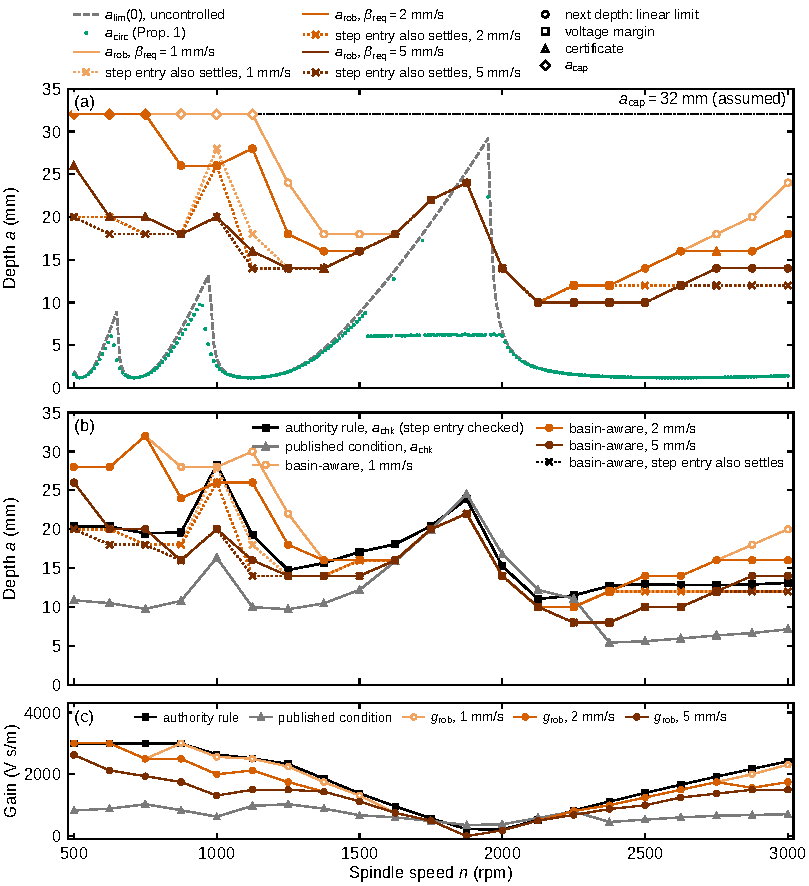
\includegraphics[width=0.86\textwidth]{figures/fig_basin_aware.pdf}
  \caption{Basin-aware stability chart. (a)~Largest depth $a_{\mathrm{rob}}$ up to which every grid depth is linearly stable, keeps \SI{10}{\percent} of the voltage free and has a certified kick of at least $\beta_{\mathrm{req}}=1$, 2 or \SI{5}{\milli\metre\per\second} (C2, averaged collocation model), with the condition that fails at the next grid depth (markers); for comparison, the authority schedule of Section~\ref{sec:feasibility} ($g\le\SI{1500}{\volt\second\per\metre}$: linear limit and checked depth), the depth of the published condition, Eq.~\eqref{eq:pub}, the uncontrolled limit and the depth $a_{\mathrm{circ}}$ below which the averaged delay model attracts every solution at the authority gains (Proposition~\ref{prop:circle}). (b)~Basin-aware gains and the authority-schedule gain.}
  \label{fig:ba}
\end{figure}

\subsection{Validation in the simulator}\label{sec:ba-valid}

At six speeds (750, 1125, 1375, 2000, 2500 and \SI{2875}{\rpm}) the design points were simulated with the \SI{9}{\volt} clip and the full surface memory. The simulated critical kick, smallest over four phases a quarter of a tooth period apart, exceeds $\beta_{\mathrm{req}}$ by factors of at least 2.75, 2.78 and 2.27 for 1, 2 and \SI{5}{\milli\metre\per\second}, or 1.6--6.9 times the certified kick, and kicks of exactly $\beta_{\mathrm{req}}$ at all 16 phases never caused chatter (0 of 96 for each requirement). The face entry settles at every design point of the chart. The step entry from rest, however, ends in chatter at 14, 12 and 7 of the 21 design points: the chart certifies the settled cut against disturbances, not the entry, which has to be gentle (Section~\ref{sec:bistab-map}) or certified separately along $-\xi_p(0)$ (Section~\ref{sec:cert-c2}), which succeeds only at shallow depths.
% src: verification/paper/basin_aware.json (validation_summary.1/2/5: points 6, all_above_beta_req true, worst_crit_kick_over_beta_req_min 2.750/2.780/2.272, td_over_cert 1.63-6.95, kicks_of_beta_req_chattering 0 of 96; summary.*.face_entry_chatters_at_design_rpm [], step_entry_chatters_at_design_rpm 14/12/7 speeds)

\section{Delayed feedback and robustness}\label{sec:delayed}

Two questions remain for a design that rests on the free voltage: whether a control law can spend the authority on the deviation from the forced orbit alone, and how robust the free voltage and the basin are to errors in the model. The first is answered by a case study of a published delayed term, the second by a Monte Carlo study.

\subsection{A delayed term that vanishes on the forced orbit: a case study}\label{sec:delayed-law}

The DVF command of Eq.~\eqref{eq:dvf} is replaced by
\begin{equation}\label{eq:comb-law}
  u(t)=-g_1\dot x(t)-g_2\bigl[\dot x(t)-\dot x(t-T)\bigr]-k_d\bigl[x(t)-x(t-T)\bigr],
\end{equation}
clipped as before, $V=\sat_{\Vmax}(u)$, and studied with $k_d=0$ (DVF\,+\,D). In the Laplace domain $U(s)=-\bigl[s\,K(s)+k_d\,E(s)\bigr]X(s)$ with $K(s)=g_1+g_2E(s)$ and $E(s)=1-e^{-sT}$. The delayed terms vanish on every $T$-periodic motion, since $E(im\omega_T)=0$ at every tooth-passing harmonic, so the forced orbit, its command $b(t)=-g_1\dot x_p(t)$ and the free voltage $u_0$ depend on $g_1$ alone, while a deviation from the orbit meets the full law. Without loop delay $K$ is positive real and the loop passive like DVF \citep{elliott2001feedback}. The law is published: its non-invasiveness is that of Pyragas-type delayed feedback \citep{pyragas1992continuous}, applied to milling by \citet{vandewouw2015ifac} and \citet{vandijk2015ijrnc}; \citet{li2022ijamt} fed back $x(t)-x(t-T)$ to lower the actuator voltage, and delayed feedback has countered regeneration in turning \citep{mancisidor2019mechatronics} and milling \citep{du2022time,du2024ijms}. It is used here to test whether linear margin translates into tolerance of disturbances under a hard clip. The models, the certificate with the delayed terms and the robustness study are detailed in the Supplementary Material.
% src: README §13.2; src/c4_comb.py (docstring, model), src/c4_robust.py (controller); tests/test_c4_comb.py (test_comb_terms_vanish_on_the_settled_cut); paper/notes/novelty.md §1.6

Both families were designed by the authority rule of Eq.~\eqref{eq:feas}: $g_1$ is the largest gain up to \SI{3000}{\volt\second\per\metre} whose steady forced command stays within \SI{9}{\volt} up to 0.9 times the design's own linear limit, so that in effect the same gain is compared with and without the delayed term. With $g_2=\SI{2000}{\volt\second\per\metre}$ the linear limit rises by a median factor of 1.78 (1.44--2.10) over the 251 speeds (Fig.~\ref{fig:dlim}a). Much of this rise, however, lies at depths that are not usable: the limit exceeds \SI{32}{\milli\metre}, twice the cutter diameter, at 222 of the 251 speeds, against 71 for DVF, and with the depth capped at \SI{32}{\milli\metre} the median gain falls to 1.31; the cutting tests of \citet{ozsoy2026robust} went up to \SI{10}{\milli\metre}.
% src: results/c4_limits.npz (feas_g1: max |g1 - g1_DVF| = 9.7 V s/m); results/c4_summary.json (limits.feasible: d2000 ratio_to_dvf median 1.78, range 1.44-2.10); verification/paper/revision_runs.json (stored.depth_2D: d2000_above_32mm 222, dvf_above_32mm 71 of 251; median_ratio 1.781, median_ratio_capped_32mm 1.309); verification/targets/experimental_points.csv (tested depths up to 10 mm)

The clipped entries tell a different story (Fig.~\ref{fig:dlim}b). Simulated at 25 speeds with the \SI{9}{\volt} clip, the face-entry limit rises with D by a median factor of 1.72, but the step-entry limit by only 1.03 (0.98--1.27): from \SI{2100}{\rpm} upwards D changes it by at most \SI{1.1}{\milli\metre}, as this limit is set by saturation during the entry, not by damping. The band in which the outcome depends on the entry therefore widens, from a median width of 7.6 to \SI{26}{\milli\metre}. At the same forced command, adding $g_2$ to the $g_1$ of the best DVF design widens the simulated basin (worst-phase critical kick) by a median factor of only 1.14 over 22 depth--speed pairs, by about 2 where the DVF certificate almost vanishes, and by 0.96--1.16 below \SI{18}{\milli\metre}; the certified kicks lie below the simulated ones at all 89 points where a kick of up to \SI{3}{\metre\per\second} caused chatter. The term is also fragile: the phase of $E(i\omega)$ alternates between lead and lag between tooth-passing harmonics, and with assumed second modes at 400--\SI{800}{\hertz} the design with $g_2=2000$ tolerates about \SI{100}{\micro\second} of loop delay, against \SI{300}{\micro\second} for DVF; a delay error of \SI{2}{\percent} or a runout of about \SI{1}{\micro\metre} makes the term act on the forced orbit.
% src: results/c4_entry.npz (face 1.45-2.12, median 1.72; step 0.98-1.27, median 1.03; from 2100 rpm +1.08 mm at most; band widths medians 7.56 and 25.88 mm); results/c4_summary.json (validate2: same_g1_over_dvf median 1.14 over 22 pairs; same_g1_near_dvf_limit 1.79-2.59, median 2.00; below 18 mm 0.96-1.16; all_cert_below_td 89/89); results/c4_summary.json (robust.by_rpm: loop delay 300/200/100/100 us for DVF/1000/2000/4000; runout_tolerance_um g2 = 2000 1.03-2.42; tooth comb eps +2 %: limit 0.87-0.93); paper/figures/figure_numbers.json (fig10)

\begin{figure}[!tbp]
  \centering
  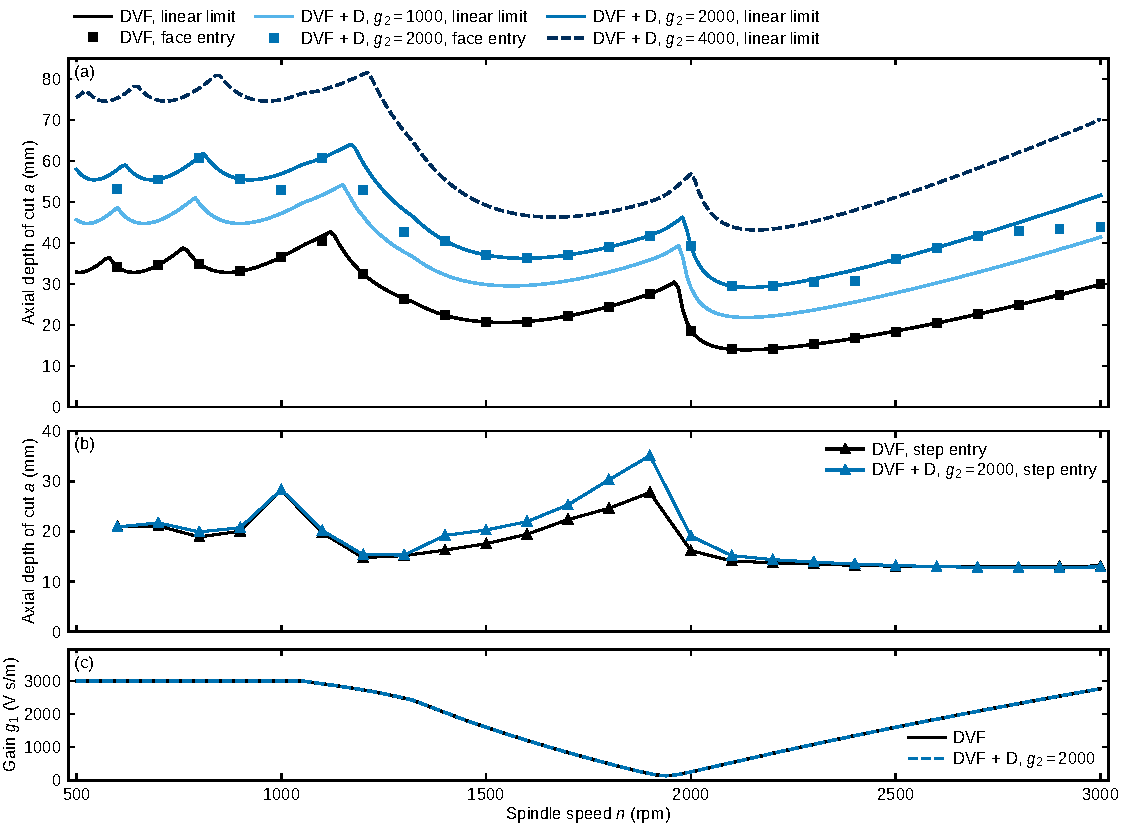
\includegraphics[width=\textwidth]{figures/fig08_delayed_limits.pdf}
  \caption{The delayed term under the same authority rule ($g_1\le\SI{3000}{\volt\second\per\metre}$; steady forced command within \SI{9}{\volt} up to 0.9 of the design's own $\alim$). (a)~Linear limits of DVF and of DVF\,+\,D with $g_2=1000$, 2000 and \SI{4000}{\volt\second\per\metre}; squares: simulated face-entry limits ($\lvert V\rvert\le\SI{9}{\volt}$, 25 speeds) of DVF and of DVF\,+\,D with $g_2=2000$; dash-dotted: $2D=\SI{32}{\milli\metre}$, twice the cutter diameter. (b)~Simulated step-entry limits of the same two designs: the linear margin gained by the delayed term hardly reaches the clipped step entry.}
  \label{fig:dlim}
\end{figure}

The case study thus gives a negative result that matters for design: a law that raises the linear limit by 78\,\% and spends no authority on the forced orbit raises the depth reached by an abrupt entry by 3\,\%, because the entry transient, not the damping of the chatter mode, saturates the actuator. Linear margin is not tolerance of disturbances.

\subsection{Robustness of the residual authority and of the basin}\label{sec:delayed-robust}

The residual authority of the nominal design was sampled under errors in the model (Table~\ref{tab:mc}). The cutting coefficients were drawn independently and uniformly within $\pm\SI{10}{\percent}$ of their nominal values (in a second case $\pm\SI{20}{\percent}$), the natural frequency within $\pm\SI{5}{\percent}$, the damping ratio within $\pm\SI{20}{\percent}$, the actuator force constant within $\pm\SI{10}{\percent}$, the eccentric runout within 0--\SI{5}{\micro\metre}, the clip level within 8.1--\SI{9}{\volt} and the loop delay within 0--\SI{300}{\micro\second}; for 4000 samples per case the linear limit and the forced command of the $g=1500$ design were computed in closed form at depths fixed as fractions of the nominal $\alim$. At the design depth $0.9\,\alim$ the sampled cut is linearly unstable in 8--\SI{20}{\percent} of the samples, and its forced orbit reaches the clip in up to \SI{9}{\percent}; at $0.98\,\alim$ the two together take 32--\SI{79}{\percent}. Even at half the limit, the forced orbit reaches the clip in 69 and \SI{50}{\percent} of the samples at 2500 and \SI{2870}{\rpm}, where the nominal residual authority is only 1.5 and \SI{3.2}{\volt} at that depth. There the runout dominates (Spearman rank correlation with $u_0$ of $-0.62$ and $-0.83$), whereas near the limit the cutting coefficient, the natural frequency and the actuator constant dominate through the linear limit itself. Widening the range of the cutting coefficients to $\pm\SI{20}{\percent}$ raises the probability of linear instability at $0.9\,\alim$ to 15--\SI{22}{\percent}. \PEND{simulated MC of the critical kick}
% src: verification/paper/mc_closed_form.json (levels.pm10/pm20.ranges; n_per_case 4000; speeds.*.fracs.*.p_unstable, p_saturated, u0_stable_median_V, dominant_u0_all, spearman_u0_all: 2500 rpm 0.5 runout -0.62, 2870 rpm 0.5 runout -0.83; nominal.u0_9V); mc_closed_form.py, mc_common.py (caches restored; nominal reproduces stored a_lim and bmax: checks.nominal)

\begin{table}[!tbp]
  \centering
  \caption{Monte Carlo of the residual authority $u_0=V_{\mathrm{clip}}-\bmax$ of the $g=\SI{1500}{\volt\second\per\metre}$ design (closed-form zero-order model; 4000 samples per case; depth fixed at a fraction of the nominal $\alim$; parameter ranges in the text). Median: over the linearly stable samples. Unstable: linearly unstable samples; clip: stable samples whose forced orbit reaches the clip ($u_0\le0$). These are frequencies over an assumed distribution, not a guarantee.}
  \label{tab:mc}
  \small
  \begin{tabular}{@{}rcccccrr@{}}
    \toprule
    Speed & $a/\alim$ & \multicolumn{1}{c}{Nominal} & \multicolumn{3}{c}{Cutting coefficients $\pm\SI{10}{\percent}$} & \multicolumn{2}{c}{$\pm\SI{20}{\percent}$}\\
    \cmidrule(lr){4-6}\cmidrule(l){7-8}
    (rpm) & & $u_0$ (\si{\volt}) & median $u_0$ (\si{\volt}) & unstable (\si{\percent}) & clip (\si{\percent}) & unstable (\si{\percent}) & clip (\si{\percent})\\
    \midrule
    1090 & 0.5 & 4.72 & 3.69 & 0 & 0 & 0 & 0\\
     & 0.7 & 4.65 & 3.71 & $<1$ & 0 & 1 & 0\\
     & 0.9 & 4.69 & 3.96 & 20 & 0 & 20 & 0\\
     & 0.98 & 4.01 & 3.20 & 32 & 0 & 31 & 0\\
    \addlinespace
    1420 & 0.5 & 2.68 & 1.80 & 0 & $<1$ & 0 & 2\\
     & 0.7 & 8.72 & 7.79 & 0 & 0 & 0 & 0\\
     & 0.9 & 2.91 & 1.98 & 12 & $<1$ & 22 & 1\\
     & 0.98 & 1.79 & 1.21 & 48 & 2 & 49 & 2\\
    \addlinespace
    2500 & 0.5 & 1.49 & -0.65 & 0 & 69 & 0 & 65\\
     & 0.7 & 7.76 & 6.14 & 0 & 0 & $<1$ & 0\\
     & 0.9 & 2.79 & 1.58 & 11 & 4 & 15 & 8\\
     & 0.98 & 1.13 & -0.63 & 31 & 48 & 33 & 39\\
    \addlinespace
    2870 & 0.5 & 3.24 & 0.01 & 0 & 50 & 0 & 49\\
     & 0.7 & 5.99 & 2.29 & 0 & 19 & 0 & 19\\
     & 0.9 & 6.74 & 4.12 & 8 & 9 & 15 & 7\\
     & 0.98 & 5.04 & 3.30 & 34 & 3 & 39 & 2\\
    \bottomrule
  \end{tabular}
\end{table}
% src: verification/paper/mc_closed_form.json (nominal.<rpm>.u0_9V; levels.pm10/pm20.speeds.<rpm>.fracs.<frac>: u0_stable_median_V, p_unstable, p_saturated)

\PEND{clip level 8.1 V against 9 V: critical kick and free voltage}

\section{Conclusions}\label{sec:conclusions}

Clipping the command of a velocity feedback loop at the force capacity of its proof-mass actuator changes the stability of a milling cut from a property of the linear system into a property of a basin. On the case study of \citet{ozsoy2026robust}, with a single-mode model that classifies 17 of its 19 published cutting tests as measured, the following was found.
\begin{enumerate}
\item With the step entry from rest that reproduces the published gains at high speeds, the authority test of saturation-aware gain scheduling is set by the entry transient. Bounding the steady forced command in closed form at every depth up to $0.9\,\alim$, with a time-domain check of the clipped entry, gives an entry-independent gain map; with gains up to \SI{1500}{\volt\second\per\metre} the checked depth averages \SI{15.87}{\milli\metre}. A checked depth is not a safe depth: it lies inside the bistable band at 104 of the 109 speeds where the band was found.
\item The forced orbit of the clipped loop has a bounded basin. A step entry from rest chatters below $0.97\,\alim$ at 157 of 251 speeds, whereas a face entry reaches the limit at every speed. At four speeds and $0.98\,\alim$, worst-phase kicks of 2.4--10.8\,\% of one tooth's cutting impulse (3--\SI{13}{\micro\metre} of equivalent displacement) end the cut in chatter; without the clip only kicks of \SI{0.78}{\metre\per\second} or more did so at the 16 points tested. At the limit the basin keeps a finite size, set by the voltage that the forced command leaves free.
\item Sector-condition LMIs with a dead zone that moves with the forced command give ellipsoidal inner estimates of this basin, numerically verified on collocation models of the averaged and of the time-periodic milling model. No simulated kick inside them ended in chatter; where the simulated basin was finite they are 1.5 to 28 times smaller than the simulated critical kicks, because of the certificate rather than of averaging.
\item The free voltage is small: a few micrometres of eccentric runout, and at \SI{2500}{\rpm} less than one, bring the forced command to the clip.
\item A published delayed difference term that vanishes on the forced orbit raises the linear limit by a median factor of 1.78 ($g_2=\SI{2000}{\volt\second\per\metre}$), 1.31 within twice the cutter diameter, but the step-entry limit by only 1.03; at the same forced command it widens the simulated basin by a median factor of 1.14, and it needs a loop delay of 100--\SI{200}{\micro\second} or less with the assumed second modes.
\end{enumerate}
All results are computational. Extending the certificates to the delay equation, budgeting the free voltage against runout, edge forces and noise, and testing the bistability experimentally are the next steps.


\section*{CRediT authorship contribution statement}
\textbf{[Author name]:} Conceptualization, Methodology, Software, Validation, Formal analysis, Investigation, Writing -- original draft, Writing -- review \& editing, Visualization. [To be completed by the authors.]

\section*{Declaration of competing interest}
The authors declare that they have no known competing financial interests or personal relationships that could have appeared to influence the work reported in this paper.

\section*{Funding}
[To be completed by the authors: the funding sources, or ``This research did not receive any specific grant from funding agencies in the public, commercial, or not-for-profit sectors.'']

\section*{Data availability}
The simulator, the scripts and the stored results that produce the numbers and figures of this article are available at [repository URL] [to be completed by the authors].

\section*{Declaration of generative AI and AI-assisted technologies in the manuscript preparation process}
During the preparation of this work the author(s) used Claude Code (Anthropic), an AI coding assistant, in order to draft and edit the text, the figures and the code that produces them. After using this tool, the author(s) reviewed and edited the content as needed and take(s) full responsibility for the content of the published article. The use of the same tool in the research itself, for writing and running the simulation and analysis code, is described in \ref{app:software}. [Authors: add any other AI tool used, e.g. for reviewing drafts, and check this statement against the journal's current policy before submission.]

\section*{Acknowledgements}
[To be completed by the authors.]

\appendix
\setcounter{table}{0}
\renewcommand{\theHtable}{\thetable}
\section{Time-domain simulator and its verification}\label{app:simulator}

\paragraph{Integration}
The simulator integrates Eqs.~\eqref{eq:eom}--\eqref{eq:dvf} for the state $(x,\dot x,q,\dot q)$, with the cutting force of Eq.~\eqref{eq:fcut} evaluated on the $N_t=4$ teeth and on 30 axial layers of thickness $a/30$, each represented by its mid-height. A revolution is divided into 512 steps, so that the tooth period is a whole number of steps (128), and each step is integrated by two classical fourth-order Runge--Kutta (RK4) sub-steps. The cutting force is re-evaluated at every RK4 stage: the tooth angles are advanced to the stage time, and the delayed displacement is taken from a cubic Hermite interpolant of the stored history of $x$ and $\dot x$. The usual scheme, a force computed at the start of a step and held over it, delays the force by half a step; at 512 steps per revolution it lowers the simulated stability limit by up to \SI{9}{\percent} and inflates the peak demand below \SI{1300}{\rpm} by a median factor of 1.6 (90th percentile 3.3). A run stops as divergent when $\lvert x\rvert$ exceeds \SI{1}{\centi\metre}. The entries and the kick of Section~\ref{sec:bistab-prot} are options; with all of them off the result is bit-identical to the plain step entry. The mean force of the face entry matches the integral of the slice force over the engaged arc to about $3\times10^{-3}$, and the chip of the feed ramp matches the geometric chip to $10^{-5}$.
% src: src/tdsim.c (rk4, deriv, fcut, xhist; divergence at |x| > 1e-2 m), src/tdsim.py (nsub = 2, spr = 512, nlay = 30); README §2 (held force: limit up to 9 % low; demand median 1.6x, 90th percentile 3.3x, also recomputed from results/gainmap_hold512.npz vs gainmap_main.npz below 1300 rpm: 1.64x, 3.32x), §11.2 (options, 3e-3, 1e-5); verification/c1/reference_defaults.json

\paragraph{Full surface memory}
For each of the 512 angular slots of every layer the simulator stores the step of the deepest pass; a pass that cuts is deeper than every earlier pass at that slot and replaces it. The chip of Eq.~\eqref{eq:chip} becomes the smaller of the chip against the last pass ($k=1$) and the chip against the deepest earlier pass at the two slots that bracket the stage angle ($k$ tooth periods back),
\begin{equation}\label{eq:surf}
  h_j=\min_{k}\Bigl[k\,f_z\sin\phi_j-\bigl(x(t)-x(t-kT)\bigr)\cos\phi_j\Bigr],
\end{equation}
and material that no earlier tooth has cut, as during the face entry, gives the fresh chip $f_z\sin\phi_j-x(t)\cos\phi_j$. The scheme was compared with a brute force that takes the least chip over the last 600 passes, which is the full memory for runs of up to 600 passes. A stable cut agrees to \SI{0.32}{\percent}, whereas single regeneration is \SI{4.9}{\percent} off, because the tool leaves the cut briefly during the entry transient. Clipped chatter is chaotic and separates pointwise, but its amplitude agrees to \SI{0.4}{\percent}, and the same run diverges (\SI{1050}{\rpm}) in both. With only the last four passes remembered, two of four chatter cases diverge where the full memory stays bounded, and a third is \SI{27}{\percent} too large.
% src: src/tdsim.c (fcut_multi, deep[], full); verification/tdsim/check9_full_memory.json (stable: 0.0032 vs brute, 0.0486 vs single; chatter amplitudes 0.5896/0.5917 and 0.4345/0.4352 mm; nreg 4: 2 diverge, 0.554 vs 0.435 mm)

\paragraph{Convergence}
The reference is the exact zero-order-hold solution of the linear loop at 8192 and 16384 steps per revolution, extrapolated to zero step (Richardson) and accurate to about \SI{0.04}{\percent} (five cases, ten revolutions each). At 512 steps per revolution the scheme deviates from it by \SI{0.74}{\percent} at \SI{500}{\rpm} ($a=\SI{1.5}{\milli\metre}$, $g=0$), by \SI{0.07}{\percent} at \SI{1950}{\rpm}, and by no more than the accuracy of the reference in the three other cases; the held-force scheme deviates by \SIrange{1.8}{8.3}{\percent}, and the 8192-step solution without extrapolation by \SIrange{0.1}{0.6}{\percent}. The peak demand at $a_{\lim}$ agrees between 512 and 8192 steps to \SI{0.18}{\percent}.
% src: verification/tdsim/check7_final_scheme.json (trajectory: rel_err_fmode1 0.0074, 0.00036, 0.000034, 0.00011, 0.00065; rel_err_fmode0 0.0176-0.0831; rel_err_zoh8192 0.0010-0.0057; rel_err_fmode1_16384 <= 0.00039; demand |rel| <= 0.0018)

\paragraph{Stability limit and layers}
An independent first-order semi-discretisation \citep{insperger2002semi,insperger2004updated,insperger2011book} with Richardson extrapolation, written separately from the code of Section~\ref{sec:model}, was compared with the ZOA limit at 12 speeds, four gains (0, 300, 800 and \SI{1500}{\volt\second\per\metre}) and both damping ratios (96 cases). With the coefficient averaged over the tooth period, which is the model of the ZOA, the largest relative difference is $2\times10^{-5}$; against a classical lobe sweep on a \SI{1}{\rpm} grid it is $6\times10^{-6}$, with no missed roots; with the time-periodic coefficient $aH(t)$ of Eq.~\eqref{eq:aHt} for the \SI{45}{\degree} helix, the ZOA is conservative by \SIrange{0}{1.04}{\percent}. With 30 layers the settled demand exceeds the closed form of Eq.~\eqref{eq:xp} by up to \SI{8.7}{\percent} at low speeds (Section~\ref{sec:feas-new}), because the layers are thicker than the axial wavelengths of the higher force harmonics; with 240 layers the difference falls within \SI{0.8}{\percent} at the three speeds checked. The layers change the peak entry demand of Eq.~\eqref{eq:pub} by $-0.03$ to $+\SI{0.85}{\percent}$ (four speeds), and their effect on the stability limit is bounded by the \SIrange{0.08}{0.73}{\percent} by which the long-run onsets below exceed the ZOA limit.
% src: verification/zoa_sdm/README.md §3-4, verification/zoa_sdm/current_grid_check.json (2.0e-5, 6.0e-6), verification/zoa_sdm/compare_12speeds.csv; README §3 (0-1.05 %); verification/feasibility/cf_vs_td_layers.json (settled, entry_peak); verification/tdsim/check8_onset_long_runs.json

\paragraph{Chatter classifier}
A settled cut converges to a $T$-periodic orbit. The classifier D1 samples $x$ once per tooth period and examines the change $\Delta x_k$ between successive samples over the second half of the window, divided into 25 blocks. A run is stable when the per-tooth growth factor fitted to the logarithm of the block RMS of $\Delta x_k$ is below $1-2\times10^{-5}$, the largest RMS of the last five blocks is below 0.98 times that of the first five, the final RMS is below that of the entry transient, and $\lvert x(t)-x(t-T)\rvert$ stays below $0.25f_z$ over the last \SI{20}{\percent} of the window, or when $\Delta x_k$ decays to round-off; a limit cycle of any size counts as chatter. After a step entry, a 300-revolution window places the time-domain limit \SIrange{0.36}{2.2}{\percent} above the ZOA limit in eight cases, whereas runs of 2000 revolutions place the onset only \SIrange{0.08}{0.73}{\percent} above it. Just above the onset, chatter saturates on a small limit cycle that the cut needs more than 300 revolutions to reach, so the shorter window biases these boundaries high by \SIrange{0.05}{1.5}{\percent}. Near the forced resonance (\SIrange{1970}{2030}{\rpm}, small gains) the 300-revolution boundaries reach 1.015--$1.05a_{\lim}$, whereas the onset lies at 1.004--$1.012a_{\lim}$, a bias of \SIrange{0.8}{4.4}{\percent}. Kick-based limits and clipped limits well below $a_{\lim}$ are not affected.
% src: src/tdboundary.py (classify_run: delta 2e-5, 25 blocks, q < 0.98, r_end < r_first, dx_end < 0.25 fz); verification/tdsim/check7_final_scheme.json (boundary: +0.36 % to +2.20 %), check8_onset_long_runs.json (onset +0.08 % to +0.73 %; bias 0.05-1.47 %), check10_forced_resonance_long_runs.json (td300 1.0149-1.05, onset 1.0039-1.0121)

\section{LMI conditions and numerical settings}\label{app:lmi}

\paragraph{Collocated model}
Writing Eq.~\eqref{eq:dev} in the state $\xi$ of Section~\ref{sec:cert-model} gives Eq.~\eqref{eq:coll} with
\begin{equation}\label{eq:app-A0}
A_0=\begin{bmatrix}
0&1&0&0&\bm 0\\
-k/m&-c/m&-K_a\omega_a^2/m&-2\zeta_a\omega_aK_a/m&\bm 0\\
0&0&0&1&\bm 0\\
0&0&-\omega_a^2&-2\zeta_a\omega_a&\bm 0\\
\hat{\bm d}_0&\bm 0&\bm 0&\bm 0&\hat D
\end{bmatrix},
\end{equation}
$B=[0,\ K_a/m,\ 0,\ 1,\ \bm 0]^\top$, where $\hat{\bm d}_0\in\mathbb R^N$ and $\hat D\in\mathbb R^{N\times N}$ are column 0 and columns $1,\dots,N$ of rows $1,\dots,N$ of $(2/T)D$, $D$ being the Chebyshev differentiation matrix on the points $\cos(\pi j/N)$, $j=0,\dots,N$ \citep{trefethen2000spectral}: the last $N$ rows state $\tfrac{\mathrm d}{\mathrm dt}\tilde x(t+\vartheta_j)=\tfrac2T\sum_{l=0}^{N}D_{jl}\,\tilde x(t+\vartheta_l)$.
% src: src/c2_certificate.py (cheb, model, history_nodes); src/c3_periodic.py (model)

\paragraph{Conditions of C2}
The program maximises $\beta$ subject to Eqs.~\eqref{eq:lmi-dec}--\eqref{eq:lmi-size}, with the left side of Eq.~\eqref{eq:lmi-dec} reduced by $\varepsilon I$, $S\ge\varepsilon$, $\varepsilon=10^{-9}$, and $\beta\ge0$. It has $n(n+1)/2+n+2$ unknowns, 326--704 for $n=4+N=24$--36, in four LMI blocks of order at most $n+1$. The decay margin is $\lambda=0.05\varrho$, $\varrho=-\max\operatorname{Re}\operatorname{eig}\mathcal A$ with $aH=\overline{aH}$, and $0.2\varrho$ when no candidate passed the check.
% src: src/c2_certificate.py (lmi: eps 1e-9, blocks M1-M4; LAM_FRAC (0.05, 0.2)); unknowns n(n+1)/2+n+2 evaluated for n = 24 and 36

\paragraph{Conditions of C3}
On segment $k$, with $W(s)$ and $Y(s)$ from Eq.~\eqref{eq:Wt}, the decrease condition~\eqref{eq:lmi-per} is imposed at the six vertices formed by $(s,\sigma)=(0,0)$, $(\tfrac12,0)$ or $(1,1)$ and $r=\pm\varepsilon_k$, as
\begin{equation}\label{eq:app-per}
\begin{bmatrix}\dot W_k-\Lambda-\Lambda^\top-2\lambda W(s) & BS_k-Y(s)^\top\\ S_kB^\top-Y(s) & 2S_k\end{bmatrix}\succ0,
\end{equation}
where $\Lambda=(A_0+BK)\,W(s)+E\,\big[\nu_0W_k+\nu_1W_{k+1}\big]$, $\nu_0=(h_k+r)(1-s)+\ell_k(s-\sigma)$ and $\nu_1=(h_k+r)s+\ell_k\sigma$; these reproduce $aH(t)W(t)$ exactly when $\sigma=s^2$. Since $E=pq^\top$ has rank one, the part of the matrix that depends on $r$ is $-r(\bar p\bar v^\top+\bar v\bar p^\top)$, with $\bar p=[p^\top\ 0]^\top$ and $\bar v=[(W(s)q)^\top\ 0]^\top$. By Petersen's lemma, exact for a scalar uncertainty \citep{petersen1987stabilization}, the matrix is positive definite for all $\lvert r\rvert\le\varepsilon_k$ if and only if, for some $\mu>0$,
\begin{equation}\label{eq:app-merged}
\begin{bmatrix}M_0-\mu\bar p\bar p^\top & \varepsilon_k\bar v\\ \varepsilon_k\bar v^\top & \mu\end{bmatrix}\succ0,
\end{equation}
with $M_0$ the matrix at $r=0$. This merges the vertices $r=\pm\varepsilon_k$, leaving three LMIs per segment; for balance, $p$ and $q$ are replaced by $p/\rho_k$ and $\rho_kq$, $\rho_k=10\,\big(\lVert p\rVert/(\lVert q\rVert\varepsilon_k)\big)^{1/2}$. At every node, Eqs.~\eqref{eq:lmi-incl}--\eqref{eq:lmi-size} are imposed with $W_k$, $Y_k$ and the level $\min(u_{0,k-1},u_{0,k})$. With $M=16$ there are $M[n(n+1)/2+n+1]+1$ unknowns and $3M$ multipliers, 7009 scalars at $N=24$. The decay margin is $0.05$, 0.02 or 0.01 times the Floquet decay rate, the next being tried when no candidate passes.
% src: src/c3_periodic.py (corners, lmi: merged block, P_SCALE 10; LAM_FRAC (0.05, 0.02, 0.01)); README §14.2, §14.9; unknowns 16 x 435 + 1 + 48 = 7009 for n = 28

\paragraph{Enclosure and command bound}
$h_k$ and $\ell_k$ are fitted to $aH$ at the midpoints of 2048 equal cells of the segment; $\varepsilon_k$ is the largest residual plus $(L+\lvert\ell_k\rvert/\tau)\,\tau/4096$, where $L\ge\lvert\mathrm d(aH)/\mathrm dt\rvert$ holds because each tooth contributes to $\mathrm d(aH)/\mathrm dt$ only through the two ends of its engaged interval in $z$. The level $u_{0,k}$ uses the largest of 257 samples of $\lvert b(t)\rvert$ on the segment, plus $\max\lvert\ddot b\rvert\,\Delta t^2/8$, plus $g$ times a bound on the forced velocity carried by the harmonics above the 40th (summed to the 20\,000th and bounded analytically beyond), with the slice-force harmonics in closed form. In C2, $\bmax$ was the largest of 4096 samples plus the same inter-sample bound, for 40 harmonics whose slice-force coefficients came from a 4096-point DFT with the entry jump on a sample; each coefficient is then off by up to \SI{4}{\newton\per\metre} and the forced command by up to \SI{5.7}{\milli\volt} pointwise at the 48 points, which, with the truncation, gives the corrections of Section~\ref{sec:cert-lmi}.
% src: src/c3_periodic.py (enclosure, aH_rate_bound, orbit, velocity_tail, lmi); src/c2_certificate.py (orbit); src/c3_summary.py (margin_errata); README §14.2, §14.9

\paragraph{Independent check}
In test (ii) of Section~\ref{sec:cert-check}, the smallest computed eigenvalue must exceed $10^3(n+1)\epsilon_{\mathrm{mach}}$ times the largest absolute eigenvalue. This margin lies well above the backward error of the symmetric eigensolver, but the test is made in floating point; it is not an interval-arithmetic proof. For C3 the test is applied at all $6M$ vertices separately, also when they were merged in the solve, with a scale that also includes $\big(\lVert A_0+BK\rVert+(\lvert\nu_0\rvert+\lvert\nu_1\rvert)\lVert E\rVert\big)\max(\lVert W_k\rVert,\lVert W_{k+1}\rVert)$ and $(\lVert W_k\rVert+\lVert W_{k+1}\rVert)/\tau$, to cover rounding in $\dot W_k$ and in $\mathcal AW$. Inclusion, validity and size are evaluated at every node through Cholesky factors, and an exceeded bound is repaired by one common scaling of all $(W_k,Y_k,S_k)$, which keeps every decrease LMI.
% src: src/c2_certificate.py (check); src/c3_periodic.py (check)

\paragraph{Settings and cost}
Table~\ref{tab:lmi-settings} lists the settings. At all 48 validation points the kept C2 candidate came from a re-centred solve. For C3, solves without the warm start needed about 200 iterations (eight segments, during development) and stopped short, while a second, re-centred pass added only 0.4\,\% at \SI{2500}{\rpm} and $0.9\alim$. Merging made the solves 3--4 times faster and agreed with separate vertices to the fifth digit (eight segments, development) and within 0.2\,\% in a test (four segments). In the first run the merged problem failed at the first solver step at 32 of the 48 points, its multiplier block mixing the small residual with terms of the size of $\mathcal A$; balancing removed this, and with the fallbacks 47 points were certified, the one at \SI{2870}{\rpm} and $0.98\alim$ only with separate vertices. At \SI{2500}{\rpm} and $0.98\alim$ the best candidates had a positive smallest eigenvalue below the round-off bound. Sizes reproduce to about 0.1\,\%, not bit for bit (3.426 against \SI{3.428}{\milli\metre\per\second} at \SI{2500}{\rpm}, $0.9\alim$).
% src: README §12.3, §14.5, §14.9; results/c2_validate.npz (msg: pass 1 or 2 at all 48 points), c3_basin.npz and c3_edge.npz (msg)

\begin{table}[!tbp]
\centering
\caption{Numerical settings and cost of the certificates; $\varrho$ is the linear decay rate (C2) or the Floquet decay rate (C3).}
\label{tab:lmi-settings}
\small
\begin{tabular}{@{}>{\raggedright\arraybackslash}p{0.17\textwidth}>{\raggedright\arraybackslash}p{0.38\textwidth}>{\raggedright\arraybackslash}p{0.38\textwidth}@{}}
\toprule
 & C2 (averaged model) & C3 (periodic model)\\
\midrule
Solver & Clarabel; gap (absolute, relative) and feasibility tolerances $10^{-10}$, at most 400 iterations (48 points, step entry); defaults (surface) & Clarabel defaults, at most 120 iterations, direct solver faer, one thread\\
Fallbacks & $\lambda=0.2\varrho$ if no candidate passes at $0.05\varrho$ (used for 4 of the 287 surface certificates) & $\lambda=0.05$, 0.02, $0.01\varrho$; static regularisation $10^{-7}$ instead of $10^{-8}$; separate vertices\\
Strictness & $\varepsilon=10^{-9}$ & $\varepsilon=10^{-9}$\\
Discretisation & $N=16+4\lceil T\omega_n/2\pi\rceil=20$--32 & as C2; $M=16$ (8 and 32 in Section~\ref{sec:cert-c3})\\
Solves & three: scaled, then two re-centred & one, in the coordinates of the C2 certificate\\
Size & 326--704 unknowns & 7009 unknowns at $N=24$\\
Time, memory & about \SI{2}{\hour} for the campaign, including its simulations, on four cores & 4--\SI{10}{\minute} per certificate, 2--5\,GB (4.7\,GB with separate vertices at $N=24$; about twice with $M=32$, 5.2\,GB at $N=20$); about \SI{8}{\hour} for the campaign on four cores\\
\bottomrule
\end{tabular}
\end{table}
% src: src/c2_certificate.py (TIGHT, FAST, LAM_FRAC, N_PASS, nodes_for); src/c3_periodic.py (SOLVER, REG_RETRY, ATTEMPTS, LAM_FRAC, N_PASS, M_C); results/c2_surface.npz (msg: lam 0.2 sigma at 4 points); README §10, §14.6, §14.9

\paragraph{Model runs used for comparison}
Critical kicks of the collocated models used the true dead zone, held over each of 256 steps per tooth period, with the linear part integrated exactly (C2) or by fourth-order Magnus propagators with two Gauss points (C3) \citep{blanes2009magnus}; a run diverged if its state norm was not finite or exceeded $10\Delta v$ after 1200 tooth periods. Logarithmic bisection on $[10^{-4},3]$\,m/s used nine steps (about 2\,\%) and the minimum over four phases in C2, and 14 steps (0.06\,\%) at each of the 16 phases in C3; the time step moves the result by about 0.1--0.2\,\%. Floquet limits used 200 Magnus steps per period and bisection to a relative $10^{-5}$; with $N+8$ nodes the spectral radius at the computed limit differs from 1 by at most $6\times10^{-6}$, and at nine speeds at half immersion the limit agrees with stored semi-discretisation limits \citep{insperger2002semi,insperger2004updated} within $1.3\times10^{-5}$ (no such check at $a_e/D=0.1$). The sampled check followed 48 trajectories per point over 40 tooth periods. The off-axis test applied the 18 boundary points (for C3, of the ellipsoid at the phase of application) at four phases a quarter of a tooth period apart, at revolution 100 of a face entry with the \SI{9}{\volt} clip, and classified the following 300 revolutions as in Section~\ref{sec:bistability}; the C2 runs used the full surface memory, the C3 runs the last four passes, as in the original campaign, their starts lying inside the validity bound.
% src: src/c2_certificate.py (run_model, model_critical_kick, proof_check, td_offaxis); src/c3_periodic.py (propagators, step_maps, model_kick_by_phase, NBIS, L_SIM, floquet_a_lim, td_offaxis); results/c3_floquet.npz (rho_n8: 4.9e-6, 5.5e-6); README §14.4, §14.9

\section{Software, reproducibility and use of AI tools}\label{app:software}

The time-domain simulator is written in C and compiled with GCC 13.3. The analyses use Python 3.13 with the libraries NumPy 2.5, SciPy 1.18 and Matplotlib 3.11, and the LMIs are solved with the interior-point solver Clarabel 0.11 \citep{goulart2024clarabel}. A solver's answer is not taken as a proof: every candidate certificate is accepted only after the eigenvalue and Cholesky tests of \ref{app:lmi}, which are computed independently of the solver. An automated test suite of 180 tests rebuilds the summary tables from the stored results and checks the main numbers reported here; the stored long simulations that support the classifier corrections of \ref{app:simulator} are part of it.

The simulation and analysis code, its tests and the scripts that draw the figures were written and run with the assistance of [name of the AI tool or service], under the direction of the author(s). [To be completed by the authors: who designed the study, which steps were checked by hand, and how.] All code, stored results and tests are available at [repository URL], so that the numbers and figures of this article can be regenerated and inspected.


\bibliographystyle{elsarticle-num-names}
\bibliography{refs}

\end{document}
